\def\year{2022}\relax
%File: formatting-instructions-latex-2022.tex
%release 2022.1
\documentclass[letterpaper]{article} % DO NOT CHANGE THIS
\usepackage{aaai22}  % DO NOT CHANGE THIS
\usepackage{times}  % DO NOT CHANGE THIS
\usepackage{helvet}  % DO NOT CHANGE THIS
\usepackage{courier}  % DO NOT CHANGE THIS
\usepackage[hyphens]{url}  % DO NOT CHANGE THIS
\usepackage{graphicx} % DO NOT CHANGE THIS
\urlstyle{rm} % DO NOT CHANGE THIS
\def\UrlFont{\rm}  % DO NOT CHANGE THIS
\usepackage{natbib}  % DO NOT CHANGE THIS AND DO NOT ADD ANY OPTIONS TO IT
\usepackage{caption} % DO NOT CHANGE THIS AND DO NOT ADD ANY OPTIONS TO IT
\DeclareCaptionStyle{ruled}{labelfont=normalfont,labelsep=colon,strut=off} % DO NOT CHANGE THIS
\frenchspacing  % DO NOT CHANGE THIS
\setlength{\pdfpagewidth}{8.5in}  % DO NOT CHANGE THIS
\setlength{\pdfpageheight}{11in}  % DO NOT CHANGE THIS
%
% These are recommended to typeset algorithms but not required. See the subsubsection on algorithms. Remove them if you don't have algorithms in your paper.
\usepackage{algorithm}
\usepackage{algorithmic}

\usepackage{graphicx, caption, subcaption}
\usepackage{amsmath}
\usepackage{color}
\usepackage{multirow}
\usepackage{booktabs}
\usepackage{bbm}
\usepackage{enumitem}
\usepackage[flushleft]{threeparttable}
\usepackage{makecell}
% \usepackage{hyperref}
\usepackage{amsfonts}
\usepackage[normalem]{ulem}
\newcommand{\KZ}[1]{\textcolor{blue}{Kenny: #1}}
\newcommand{\cut}[1]{}
%
% These are are recommended to typeset listings but not required. See the subsubsection on listing. Remove this block if you don't have listings in your paper.
\usepackage{newfloat}
\usepackage{listings}
\lstset{%
	basicstyle={\footnotesize\ttfamily},% footnotesize acceptable for monospace
	numbers=left,numberstyle=\footnotesize,xleftmargin=2em,% show line numbers, remove this entire line if you don't want the numbers.
	aboveskip=0pt,belowskip=0pt,%
	showstringspaces=false,tabsize=2,breaklines=true}
\floatstyle{ruled}
\newfloat{listing}{tb}{lst}{}
\floatname{listing}{Listing}
%
%\nocopyright
%
% PDF Info Is REQUIRED.
% For /Title, write your title in Mixed Case.
% Don't use accents or commands. Retain the parentheses.
% For /Author, add all authors within the parentheses,
% separated by commas. No accents, special characters
% or commands are allowed.
% Keep the /TemplateVersion tag as is
\pdfinfo{
/Title (Product Categorization for Multiple Evolving Businesses)
/Author (AAAI Press Staff, Pater Patel Schneider, Sunil Issar, J. Scott Penberthy, George Ferguson, Hans Guesgen, Francisco Cruz, Marc Pujol-Gonzalez)
/TemplateVersion (2022.1)
}

% DISALLOWED PACKAGES
% \usepackage{authblk} -- This package is specifically forbidden
% \usepackage{balance} -- This package is specifically forbidden
% \usepackage{color (if used in text)
% \usepackage{CJK} -- This package is specifically forbidden
% \usepackage{float} -- This package is specifically forbidden
% \usepackage{flushend} -- This package is specifically forbidden
% \usepackage{fontenc} -- This package is specifically forbidden
% \usepackage{fullpage} -- This package is specifically forbidden
% \usepackage{geometry} -- This package is specifically forbidden
% \usepackage{grffile} -- This package is specifically forbidden
% \usepackage{hyperref} -- This package is specifically forbidden
% \usepackage{navigator} -- This package is specifically forbidden
% (or any other package that embeds links such as navigator or hyperref)
% \indentfirst} -- This package is specifically forbidden
% \layout} -- This package is specifically forbidden
% \multicol} -- This package is specifically forbidden
% \nameref} -- This package is specifically forbidden
% \usepackage{savetrees} -- This package is specifically forbidden
% \usepackage{setspace} -- This package is specifically forbidden
% \usepackage{stfloats} -- This package is specifically forbidden
% \usepackage{tabu} -- This package is specifically forbidden
% \usepackage{titlesec} -- This package is specifically forbidden
% \usepackage{tocbibind} -- This package is specifically forbidden
% \usepackage{ulem} -- This package is specifically forbidden
% \usepackage{wrapfig} -- This package is specifically forbidden
% DISALLOWED COMMANDS
% \nocopyright -- Your paper will not be published if you use this command
% \addtolength -- This command may not be used
% \balance -- This command may not be used
% \baselinestretch -- Your paper will not be published if you use this command
% \clearpage -- No page breaks of any kind may be used for the final version of your paper
% \columnsep -- This command may not be used
% \newpage -- No page breaks of any kind may be used for the final version of your paper
% \pagebreak -- No page breaks of any kind may be used for the final version of your paperr
% \pagestyle -- This command may not be used
% \tiny -- This is not an acceptable font size.
% \vspace{- -- No negative value may be used in proximity of a caption, figure, table, section, subsection, subsubsection, or reference
% \vskip{- -- No negative value may be used to alter spacing above or below a caption, figure, table, section, subsection, subsubsection, or reference

\setcounter{secnumdepth}{2} %May be changed to 1 or 2 if section numbers are desired.

% The file aaai22.sty is the style file for AAAI Press
% proceedings, working notes, and technical reports.
%

% Title

% Your title must be in mixed case, not sentence case.
% That means all verbs (including short verbs like be, is, using,and go),
% nouns, adverbs, adjectives should be capitalized, including both words in hyphenated terms, while
% articles, conjunctions, and prepositions are lower case unless they
% directly follow a colon or long dash
\title{Enhanced Semantic Space: Integrate Concepts \\to Unify Dynamic Multi-Domain Product Categorization}
\author{
    %Authors
    % All authors must be in the same font size and format.
    % Written by AAAI Press Staff\textsuperscript{\rm 1}\thanks{With help from the AAAI Publications Committee.}\\
    Submission ID: 8044
    % AAAI Style Contributions by Pater Patel Schneider,
    % Sunil Issar,\\
    % J. Scott Penberthy,
    % George Ferguson,
    % Hans Guesgen,
    % Francisco Cruz\equalcontrib,
    % Marc Pujol-Gonzalez\equalcontrib
}
% \affiliations{
%     %Afiliations
%     \textsuperscript{\rm 1}Association for the Advancement of Artificial Intelligence\\
%     % If you have multiple authors and multiple affiliations
%     % use superscripts in text and roman font to identify them.
%     % For example,

%     % Sunil Issar, \textsuperscript{\rm 2}
%     % J. Scott Penberthy, \textsuperscript{\rm 3}
%     % George Ferguson,\textsuperscript{\rm 4}
%     % Hans Guesgen, \textsuperscript{\rm 5}.
%     % Note that the comma should be placed BEFORE the superscript for optimum readability

%     2275 East Bayshore Road, Suite 160\\
%     Palo Alto, California 94303\\
%     % email address must be in roman text type, not monospace or sans serif
%     publications22@aaai.org
% %
% % See more examples next
% }

% %Example, Single Author, ->> remove \iffalse,\fi and place them surrounding AAAI title to use it
% \iffalse
% \title{My Publication Title --- Single Author}
% \author {
%     Author Name
% }
% \affiliations{
%     Affiliation\\
%     Affiliation Line 2\\
%     name@example.com
% }
% \fi

% \iffalse
% %Example, Multiple Authors, ->> remove \iffalse,\fi and place them surrounding AAAI title to use it
% \title{My Publication Title --- Multiple Authors}
% \author {
%     % Authors
%     First Author Name,\textsuperscript{\rm 1}
%     Second Author Name, \textsuperscript{\rm 2}
%     Third Author Name \textsuperscript{\rm 1}
% }
% \affiliations {
%     % Affiliations
%     \textsuperscript{\rm 1} Affiliation 1\\
%     \textsuperscript{\rm 2} Affiliation 2\\
%     firstAuthor@affiliation1.com, secondAuthor@affilation2.com, thirdAuthor@affiliation1.com
% }
% \fi


% REMOVE THIS: bibentry
% This is only needed to show inline citations in the guidelines document. You should not need it and can safely delete it.
\usepackage{bibentry}
% END REMOVE bibentry

\newcommand{\TODO}[1]{\textcolor{red}{(todo: #1)}}
\newcommand{\secref}[1]{Section \ref{#1}}
\newcommand{\figref}[1]{Figure \ref{#1}}
\newcommand{\eqnref}[1]{Eq. (\ref{#1})}
\newcommand{\tabref}[1]{Table \ref{#1}}
\newcommand{\exref}[1]{Example \ref{#1}}
\newcommand{\tabincell}[2]{\begin{tabular}{@{}#1@{}}#2\end{tabular}}

\begin{document}

\maketitle

\begin{abstract}
    Product categorization is to assign a product with a suitable category, which is usually organized in a predefined taxonomy.
    As e-commerce platforms developing different business lines, a special but challenging categorization scenario emerges, where there are multiple domain-specific category taxonomies and each of them evolves dynamically over time. 
    In order to unify the categorization process and jointly utilize the cross-domain data, we propose a two-stage taxonomy-agnostic framework that relies solely on calculating the semantic relatedness 
    between product titles and category names in the vector space. 
    However, pure vector matching may fall for the surface form of text, 
    % \textbf{indulges the surface form of the text dominating the score model}, 
    and we thus further leverage the universal ``knowledge'' across different business domains to complement textual semantics.
    % to mitigate this issue. 
    We design a heuristic retrieval strategy and pretrain a contrastive ranking model with the help of ``concept'', which resembles the shared keyword knowledge cross domains. 
    % In the end, the semantic matching is the backbone of our framework, but the concept knowledge is the fuel to power the unified model. 
    Our comprehensive experiments show that our method outperforms existing sophisticated approaches quantitatively and efficiently on dynamical multi-domain taxonomies. 
\end{abstract}

%\IEEEraisesectionheading{
% %\IEEEraisesectionheading{
% %\IEEEraisesectionheading{
% \input{intro}
\section{Introduction}\label{sec:intro}
 %}
% \section{Introduction}\label{sec:intro}

% \begin{enumerate}
% \item Motivation: application scenarios (with 1-2 running examples);
% \item Characteristics of the data sources and their challenges;
% \item Briefly introduce previous approaches to extract information 
% from images including setting the document zone, and their limitations.
% \item General flow of our approach (may give a diagram here)
% \end{enumerate}
% scenary

Due to ever evolving hardware and software, many medical images
such as electro-cardio graphs (ECGs), X-ray or ultrasound images  
are directly printed and stored in hard copy formats. 
% \KZ{Insert 4 example images here.}
%Examples are shown in \figref{fig:medicalImages}. 
% These images often contain a mix of graphics and text, which
% include parameter settings of the hardware, test measurements or simple
% diagnosis. 
These images often contain a mix of graphics and text, which 
include technical settings of the hardware used, test measurements or simple diagnoses.
Recently, there has been a growing demand for digitizing such 
medical information from paper media sources, especially legacy ones, or patients who want to keep track of these documents by themselves digitally. 
Apart from scanning the graphics into a digital format, extracting 
the semi-structured textual information is also an important part of
building electronic medical records for patients. 

%\begin{figure}[!htb]
%\centering
%\subfloat[ECG]{
%\label{fig:medicalimage:ecg}
%\epsfig{file=figure/17_ori.eps, width=0.4\columnwidth}
%}
%% \hfill
%\subfloat[MRI]{
%	\label{fig:medicalimage:mrt}
%	\epsfig{file=figure/MRI.eps, width=0.4\columnwidth}
%}
%\\
%\subfloat[X-RAY]{
%\label{fig:medicalimage:xray}
%\epsfig{file=figure/X-RAY.eps, width=0.4\columnwidth}
%}
%%\hfill
%\subfloat[EEG]{
%\label{fig:medicalimage:eeg}
%\epsfig{file=figure/EEG.eps, width=0.4\columnwidth}
%}
%\caption{Examples of Medical Images}
%\label{fig:medicalImages}
%\end{figure}

Optical character recognition (OCR)  \cite{mori1992historical,smith2007overview} is 
a traditional technique used to turn images of printed text into machine encoded
text. It is well researched and performs well on plain text 
documents such as novels and reports, for a variety of languages. 
%For example, Tesseract, which is one of 
%the most popular open source multilingual recognizers, logs an error 
%rate of 3.72\% for English words and 3.77\% for simplified 
%Chinese characters\cite{smith2009adapting}. 
%Google Books \cite{googlebooks} and Gutenberg \cite{gutenberg} are
%projects which have scanned a large number of paper books into text for free and open
%access. These projects made exclusive use of OCR for this conversion and 
%achieved high accuracy \cite{vincent2007google} \cite{lebert2008project}. 
% 99\% for Gutenberg project \cite{lebert2008project}. 
% \KZ{Give the accuracy of google and gutenberg if available.}


\begin{figure}[th]
\centering
\epsfig{file=figure/17_b.eps, width=0.8\columnwidth}
\caption{An ECG image with text area (red circle) of interest.}
\label{fig:ecgexample2}
\end{figure}

For a semi-structured medical image, such as 
\figref{fig:ecgexample2}, we would like to extract the attribute-value 
pairs (e.g., {\em Vent. rate = 63 bpm}) and possibly other values such as
date ({\em 18-Nov-2010}) and time ({\em 9:13:02}) since those values endow us with lots of information about the patient. 
Existing OCR software cannot extract such structured information in a straightforward 
fashion, 
but instead it produces rather convoluted results from the whole image, 
similar to those in \figref{fig:ocrre}, which was produced by Tesseract, 
a popular multi-lingual recognizers. 
% \KZ{Maybe include the x-y coordinate info in the output as well?}  

\begin{figure}[th]
\centering
\scriptsize
\begin{verbatim}
<p class="ocr_par" title="box 263 33 444 119">
   <span class="ocr_l" title="box 264 33 336 45">
       <span class="ocrx_w" title="box 264 33 299 45">Vcnt.</span> 
       <span class="ocrx_w" title="box 308 34 336 45">rule</span> 
   </span>
   <span class='ocr_l'>
       <span class="ocrx_w" title="box 264 51 283 64">PR</span> 
       <span class="ocrx_w" title="box 291 51 346 64">Interval</span> 
       <span class="ocrx_w" title="box 389 52 411 64">140</span> 
       <span class="ocrx_w" title="box 420 55 439 64">ms</span> 
   </span>
   ...
   </span>
</p>
<p class="ocr_p" dir="ltr">
   <span class="ocr_l">
       <span class="ocrx_w" title="box 396 33 411 45">53</span> 
       <span class="ocrx_w" title="box 420 33 449 48">bpm</span> 
   </span>
</p>
\end{verbatim}
\caption{Snippet OCR results in XML, input to our framework.}
\label{fig:ocrre}
\end{figure}


%\input{xmlre1}

%However, OCR alone does not work well on semi-structured text and hence
%can't be directly used for information extraction from the aforementioned
%medical images. \KZ{Give the reason here, perhaps because OCR models are
%largely Markov based? So semi-structured data breaks the flow of text.}
%When a medical image is input to an ordinary OCR software, the spatial 
%information of the text components is often lost or mixed with noises
%and errors.
%%The reason is OCR converts the whole images into text data, in which 
%%useful information often mix with noises and errors. 
%In this paper, we would like to extract the attribute-value pairs
%and possibly other values from \figref{fig:ecgexample1} 
%and \figref{fig:ecgexample2}. 
%% or medical ultrasonography report. 
%Such images contain lots of non-textual information or noises.

% example & ref
%\begin{figure}[ht]
%\centering
%\epsfig{file=figure/46.eps, width=0.8\columnwidth}
%\caption{ECG Images From Printer1}
%\label{fig:ecgexample1}
%\end{figure}

% \begin{figure}[ht]
% \centering
% \subfloat[Printer1]{
% \label{fig:ecgexample:a}
% \epsfig{file=figure/46.eps, width=0.48\columnwidth}
% }
% \hfill
% \subfloat[Printer2]{
% \label{fig:ecgexample:b}
% \epsfig{file=figure/17.eps, width=0.48\columnwidth}
% }
% \caption{ECG images from two different printers}
% \label{fig:ecgexample}
% \end{figure}

Also, errors in the OCR text \cite{darwish2007error,taghva1996evaluation} will greatly affect the effectiveness 
of other related tasks. Much work has been done to improve the performance of the OCR\cite{kolak2003generative,cesarini1998informys}. However, there are still a number of significant challenges involved in extracting the information from medical images or OCR results in XML form. 

% First, medical images differ from pure text document in that them have 
% layout information. 
First, medical images differ from pure text documents in that 
they contain layout information.
Although most current OCR engines attempt to reproduce the physical 
layout of the text units, 
%(along with X-Y coordinates) and store them 
%in a special format such as XML 
% (\KZ{Better in the previous example})
such spatial
information is approximate and sometimes inaccurate, which is why neighboring
text blocks in \figref{fig:ecgexample2}, such as ``Vent. Rate'' and
``63 bpm'' were not automatically combined into the same XML block, but were 
rather far apart (shown in two different ``classes'') in \figref{fig:ocrre} made by OCR softwares. 
%Even for images produced by the same ECG printer, 
%the XML results can still be very different as 
The spatial layout is sensitive to many factors, such as accidental spots 
on the prints, color and contrast, or the angle of the camera. 
%In this case, solutions for other application domains, for example, the web, 
%are not well suited for information extraction from printed documents \cite{bartoli2014semisupervised}. With such inaccurate
%layout information produced by OCR,
%it is not easy to write a simple wrapper program to extract useful
%data from images, even if the images come from the same printer. 

%Writing a wrapper for each
%individual image would be tedious and counter-productive. Therefore,
%a mechanism that makes use of the spatial locality of the 
%text units in the image and 
%accommodates slight variations in the spatial layout would make the extraction
%more accurate and fault-tolerant.

%For example, \figref{fig:ocrre} is the simplified OCR results for the ECGs in 
%\figref{fig:ecgexample1} and \figref{fig:ecgexample2}. The results are in the XML format and have attritube named {\em class} 
%for layout information. Although these two images share similar format. 
%OCR engine generates different results in that it splits elements that 
%should be in the same line into two lines in the second example. 
%XML is sensitive to the layout results so it's hard to tolerate 
%all the layout results. 
%
% example check the term
% layout of ocr results can be restore, so why OCR engine don't restore the results 
% using the similar methods as we do?
% or the way we handle the layout problem is quite simple

% Delete for TIP
% Second, exiting OCR engines make heavy use of Markov properties such as n-grams
% since they primarily target the transformation of large body of text 
% \cite{kolak2003generative}. 
% % \KZ{Needs some refs here.}
% Unfortunately, the semi-structured texts in medical images are often 
% short and not even written in complete sentences, thus breaking Markov assumption. To make
% matters worse, medical images contain scientific language, which may be
% very different from the training corpora of these OCR engines.
% This explains why we see errors like ``Vcnt'' and ``rule'' 
% in \figref{fig:ocrre}. 
% %can't guarantee a perfect performance, which means 
% %there are errors and noises in the OCR results.
% %Many of them due to the fact that the data are no longer long, continous
% %sentences, thus breaking the Markov assumption made by many OCR algorithms. 
% %In \figref{fig:ocrresub:b}, ``Vent." is misrecognized as ``Vcnt.". 
% Without sufficient contextual information, OCR may also misrecognize a 
% digit as an alphabetic character, or as another similar digit. 
% Furthermore, the mix of text with images and formatting
% lines often confuses the OCR engine, which is more biased toward full
% text images.
% Exact pattern matching, as used in
% traditional information extraction, doesn't work with such noisy OCR output
% as it doesn't tolerate noises or errors in text. 
% %It's hard to autocorrect these errors 
% %because image quality is the most important affecting factor. 
% %The text we are processing can be full of no meaning words or 
% %strange numbers. 
% A fuzzy matching strategy is more desirable in this case. 
% % example, what are the traditional IEs

Second, there are many types of medical images, resulting from a variety of
medical tests. Different equipments for the same test can produce vastly 
different images. Writing individual extraction wrappers 
for the OCR outputs of all these formats is tedious and inefficient, 
and difficult for non-programmers.
%not to mention that there are significant programming barriers for 
%writing these wrappers, especially for the medical professionals who are the
%end users of these extraction results. 
%A more user-friendly approach enabling users to specify such extraction requirements would be preferred. 
%There are various kinds of medical images, such as electrocardiograph report, 
%medical ultrasonography report, etc. 
%However the basic measures for each type of medical test (e.g., ECG), 
%are very similar from machine to machine. Only the layouts are 
%different. 
% example medical images

Finally, most off-the-shelf OCR programs are pre-trained with specific 
recognition models, which may not be suitable for the extraction of 
%medical images.
%Furthermore, changes in imaging equipment technology over time may produce 
%different formats, layout, or terminology, rendering existing OCR models 
%obsolete. 
Re-training the models requires a large amount of labeled data, which may
not be available. 
%Incremental training as more labeled data arrives
%is currently not supported by any OCR product.    

%There have been some limited attempts to address some of the above challenges. 
%One solution is a plugin of an OCR program that allows the user to specify 
%target zones of interest in the image to be extracted. The zones specified for
%one image can be applied to images with slight variations by adjusting against
%a fixed reference point that is supposed to exist in all these images.
%% \KZ{I think the problem is not so much with the zones, because we also
%% have zones, but rather with the reference point.}
%% \JY{}
%% example products
%% http://www.square-9.com/automated-data-extraction-optical-character-recognition
%The problem with this solution is its high reliance on the OCR zones  
%established by the user. The performance of the results is affected by the 
%accuracy of the zones. If the zones are too big, the results will be full of 
%noise. If the zones are too small, results will miss something. 
%
%Another solution involves using the page layout analysis technique. The page layout 
%analysis technique is used to determine where the text 
%resides on a page \cite{o1993document}, 
%% \KZ{This page layout analysis approach is not clearly described. I don't understand after reading this paragraph.}
%% By using page layout analysis technique, the hierarchy of physical components 
%% can be generated and to match with the hierarchy of logical components, which 
%% is predefined. 
%this includes identifying and categorizing the 
%regions of interest in the scanned image of a text document. 
%Typically, the first step is to segment text zones from 
%non-textual zones and arrange them in their original order. 
%Then in order to analyze the logical roles of the text zones 
%(titles, captions, footnotes, etc.), logical layout analysis 
%is used for labeling the semantics of the text zones.
%Generally, page layout analysis is used for documents. The problem with applying 
%such a technique on medical images is that it creates so much noises 
%that performance is ultimately affected. 
%For medical imaging reports like ECG, useful information is often 
%found in the small components of the image, while most of the images are 
%read as noises. 
% check paper and more description, weakness, ref

%In this paper, 
%we propose a spatial data description language, which borrows its syntax from
%PADS \cite{fisher+:pads}, an ad hoc data processing language, 
%for describing semi-structured data in medical images. 
%% ref
%We call this language OCR description language, or ODL. 
%ODL is designed for extracting and parsing semi-structured text data 
%from images. We believe that  information extraction from those data in ODL form may be much easier than extracting information from rough data or data in XML form, which means that our preprocessing part proves to be necessary.
%%An example ODL description for the image in 
%%\figref{fig:ecgexample2} is shown in 
%%\figref{fig:description}. \KZ{Make this description two column, and give
%%some brief explanation of this description here.} 
%%The parsing result of this description is shown
%%in \figref{fig:parsing result}. \KZ{Give some explanation of the results,
%%otherwise don't show the result here. E.g., you need to explain what F, E, etc.
%%mean. You want to say that even though rate has been recognized as rule,
%%the bpm value was still extracted (but still wrong!).}
%% \KZ{I removed the preprocessing part, cos it's not important. Talk about it in
%% discussion sec.}
%%The our approach starts by preprocessing the images for text results.
%To use this framework, the user first describes the components in the image
%that he or she is interested in extracting. This includes constant strings
%and variables of different data types.   
%ODL allows the user to specify the approximate spatial layout and constraints on
%the data, e.g., integers within 
%a certain range, real numbers with certain decimal points, etc. 
%%This information is then as the key component in our fuzzy matching strategy. 
%The system then automatically generates a parser for these medical images.
%This parser uses the output XML from OCR with spatial information as an input, 
%and outputs a data structure with values extracted for each variables
%in the description, unless there is an unrecoverable error during the parsing process.
%In addition, approximate layout information and constraints are used in parsing process 
%to tolerate noises and small format variations in the input images. 
%%Specifically, this method could be called fuzzy matching, meaning that more candidates could be saved after the parsing process.  It's obvious that we may have a higher probability to obtain the accurate result if more candidates are kept so that fuzzy match should be used properly in our system.
%%An autogenerated parser based on the ODL description can release us from 
%%repetitive work. In this way, we turn the task of writing complex parsers 
%%into describing information on images.
%
%
%When users process many images of the same format, the system 
%automatically discovers parsing errors given the current model and 
%prompts the user to manually correct some of the frequent and prominent
%errors, which effectively serves as an online labeling function. 
%These incrementally labeled data are then used to update the parsing model. 


%It should be emphasized that the incremental learning model is very important in our whole system. Incremental learning is a machine learning paradigm where the learning process takes place whenever we have new examples or data added to our baisc data set, leading to a most striking difference between incremental learning and traditional machine learning: it does not assume the availability of a sufficient training set before the learning process. What incremental learning in our system is really impressive: it does not require a relatively good and stable training set at first time. In fact, it could improve the parsing result with even relatively rough training sets at first by absorbing new data or corrective information as time passes in dynamic systems. Besides, the process would be very effective when there are some new images coming in since training process would not learn from scratch, which might waste time and computation resource.

%At last, we propose an incrementally human correction framwork which can 
%make the best use of human correction to handle the misrecognition problem. 
% Base on our experiments on about 500 real life ECG images, 
% our approach achieves p1 and p2 after p3 times human correction. 
% experimental results

% \begin{figure}[h]
% \begin{lstlisting}
% Oenum str_month_t{
% 	"Jan", "Feb", "Mar", "Apr",
% 	"May", "Jun", "Jul", "Aug",
% 	"Sept", "Oct", "Nov", "Dec"
% };

% Ounion month_t{
% 	Oint(1,12)	num;
% 	str_month_t	str;
% };

% Ostruct time_t{
% 	Oint(1,31)	day;
% 	"-";
% 	month_t	month;
% 	"-";
% 	Oint	year;
% };

% Ostruct triple_t{
% 	"Vent.";
% 	hskip(\s)	skip1;
% 	"rate";
% 	Oint x;
% 	"bpm";
% 	vskip(\n)	skip2;
% };

% Oscource Ostruct entry_t{
% 	time_t(<-,-,-,0.3l>) t;
% 	triple_t(<0.1w,-,0.5w,->) d;
% };
% \end{lstlisting}
% \caption{Description}\label{fig:description}
% \end{figure}


In order to solve above problems, We design a system which makes three main contributions:
\begin{enumerate}
\item Based on some previous work on data description language \cite{lamport1986document,taft1999post,fisher+:pads},we design a new declarative spatial data description language called \textit{OCR description language}, or ODL,
which allows users to specify spatial and data constraints in medical 
images(\secref{sec:syntax});
\item We propose a noise-tolerant parser which takes OCR results
the ODL description as input and outputs a data structure with values 
extracted for each variables in the description (\secref{sec:semantics});
\item We propose an incremental manual correction 
framework\cite{von2008recaptcha,zhu2012learnpads++}, which 
takes advantage of user corrections  and improves the productivity
significantly (\secref{sec:correction}).
%To be more specific, the framework improves the traditional machine learning methods by using a incremental learning process to avoid starting from scratch when we are trying to apply human corrections in the system. That means the framework would be more effective than most corrective systems.
\end{enumerate}


\section{Introduction}\label{sec:intro}
 %}
% \section{Introduction}\label{sec:intro}

% \begin{enumerate}
% \item Motivation: application scenarios (with 1-2 running examples);
% \item Characteristics of the data sources and their challenges;
% \item Briefly introduce previous approaches to extract information 
% from images including setting the document zone, and their limitations.
% \item General flow of our approach (may give a diagram here)
% \end{enumerate}
% scenary

Due to ever evolving hardware and software, many medical images
such as electro-cardio graphs (ECGs), X-ray or ultrasound images  
are directly printed and stored in hard copy formats. 
% \KZ{Insert 4 example images here.}
%Examples are shown in \figref{fig:medicalImages}. 
% These images often contain a mix of graphics and text, which
% include parameter settings of the hardware, test measurements or simple
% diagnosis. 
These images often contain a mix of graphics and text, which 
include technical settings of the hardware used, test measurements or simple diagnoses.
Recently, there has been a growing demand for digitizing such 
medical information from paper media sources, especially legacy ones, or patients who want to keep track of these documents by themselves digitally. 
Apart from scanning the graphics into a digital format, extracting 
the semi-structured textual information is also an important part of
building electronic medical records for patients. 

%\begin{figure}[!htb]
%\centering
%\subfloat[ECG]{
%\label{fig:medicalimage:ecg}
%\epsfig{file=figure/17_ori.eps, width=0.4\columnwidth}
%}
%% \hfill
%\subfloat[MRI]{
%	\label{fig:medicalimage:mrt}
%	\epsfig{file=figure/MRI.eps, width=0.4\columnwidth}
%}
%\\
%\subfloat[X-RAY]{
%\label{fig:medicalimage:xray}
%\epsfig{file=figure/X-RAY.eps, width=0.4\columnwidth}
%}
%%\hfill
%\subfloat[EEG]{
%\label{fig:medicalimage:eeg}
%\epsfig{file=figure/EEG.eps, width=0.4\columnwidth}
%}
%\caption{Examples of Medical Images}
%\label{fig:medicalImages}
%\end{figure}

Optical character recognition (OCR)  \cite{mori1992historical,smith2007overview} is 
a traditional technique used to turn images of printed text into machine encoded
text. It is well researched and performs well on plain text 
documents such as novels and reports, for a variety of languages. 
%For example, Tesseract, which is one of 
%the most popular open source multilingual recognizers, logs an error 
%rate of 3.72\% for English words and 3.77\% for simplified 
%Chinese characters\cite{smith2009adapting}. 
%Google Books \cite{googlebooks} and Gutenberg \cite{gutenberg} are
%projects which have scanned a large number of paper books into text for free and open
%access. These projects made exclusive use of OCR for this conversion and 
%achieved high accuracy \cite{vincent2007google} \cite{lebert2008project}. 
% 99\% for Gutenberg project \cite{lebert2008project}. 
% \KZ{Give the accuracy of google and gutenberg if available.}


\begin{figure}[th]
\centering
\epsfig{file=figure/17_b.eps, width=0.8\columnwidth}
\caption{An ECG image with text area (red circle) of interest.}
\label{fig:ecgexample2}
\end{figure}

For a semi-structured medical image, such as 
\figref{fig:ecgexample2}, we would like to extract the attribute-value 
pairs (e.g., {\em Vent. rate = 63 bpm}) and possibly other values such as
date ({\em 18-Nov-2010}) and time ({\em 9:13:02}) since those values endow us with lots of information about the patient. 
Existing OCR software cannot extract such structured information in a straightforward 
fashion, 
but instead it produces rather convoluted results from the whole image, 
similar to those in \figref{fig:ocrre}, which was produced by Tesseract, 
a popular multi-lingual recognizers. 
% \KZ{Maybe include the x-y coordinate info in the output as well?}  

\begin{figure}[th]
\centering
\scriptsize
\begin{verbatim}
<p class="ocr_par" title="box 263 33 444 119">
   <span class="ocr_l" title="box 264 33 336 45">
       <span class="ocrx_w" title="box 264 33 299 45">Vcnt.</span> 
       <span class="ocrx_w" title="box 308 34 336 45">rule</span> 
   </span>
   <span class='ocr_l'>
       <span class="ocrx_w" title="box 264 51 283 64">PR</span> 
       <span class="ocrx_w" title="box 291 51 346 64">Interval</span> 
       <span class="ocrx_w" title="box 389 52 411 64">140</span> 
       <span class="ocrx_w" title="box 420 55 439 64">ms</span> 
   </span>
   ...
   </span>
</p>
<p class="ocr_p" dir="ltr">
   <span class="ocr_l">
       <span class="ocrx_w" title="box 396 33 411 45">53</span> 
       <span class="ocrx_w" title="box 420 33 449 48">bpm</span> 
   </span>
</p>
\end{verbatim}
\caption{Snippet OCR results in XML, input to our framework.}
\label{fig:ocrre}
\end{figure}


%% \begin{figure}[ht]
% \centering
% \subfigure[]{
% \label{fig:subfig:a}
% \begin{minipage}[b]{0.2\textwidth}
%\newsavebox{\firstlisting}
%\begin{lrbox}{\firstlisting}% Store first listing
%\begin{lstlisting}
%<p class='ocr_par' dir='ltr'>
%   <span class='ocr_line' id='line_2'>
%       <span class='ocrx_word' id='word_6'>Vent.</span>
%       <span class='ocrx_word' id='word_7'>rate</span>
%       <span class='ocrx_word' id='word_8'>65</span>
%       <span class='ocrx_word' id='word_9'>bpm</span>
%   </span>
%   <span class='ocr_line' id='line_3'>
%       <span class='ocrx_word' id='word_14'>PR</span>
%       <span class='ocrx_word' id='word_15'>interval</span>
%       <span class='ocrx_word' id='word_16'>162</span>
%       <span class='ocrx_word' id='word_17'>ms</span>
%   </span>
%    ...
%</p>
%\end{lstlisting}
%\end{lrbox}
% \end{minipage}
% }
% \hspace[1in]
% \subfigure[]{
% % \label{fig:subfig:b}
% % \begin{minipage}[b]{0.2\textwidth}
\newsavebox{\secondlisting}
\begin{lrbox}{\secondlisting}
% \tiny
\begin{lstlisting}[basicstyle=\tiny,]
<p class="ocr_par" title="box 263 33 444 119">
   <span class="ocr_l" title="box 264 33 336 45">
       <span class="ocrx_w" title="box 264 33 299 45">Vcnt.</span>
       <span class="ocrx_w" title="box 308 34 336 45">rule</span>
   </span>
   <span class='ocr_l'>
       <span class="ocrx_w" title="box 264 51 283 64">PR</span>
       <span class="ocrx_w" title="box 291 51 346 64">Interval</span>
       <span class="ocrx_w" title="box 389 52 411 64">140</span>
       <span class="ocrx_w" title="box 420 55 439 64">ms</span>
   </span>
   ...
   </span>
</p>
<p class="ocr_p" dir="ltr">
   <span class="ocr_l">
       <span class="ocrx_w" title="box 396 33 411 45">53</span>
       <span class="ocrx_w" title="box 420 33 449 48">bpm</span>
   </span>
</p>
\end{lstlisting}
\end{lrbox}
% % \end{minipage}
% }

% \KZ{\figref{fig:ocrre} is output from what software? Tesseract?}
\begin{figure*}[th]
%\subfloat[Image From Printer1]{
%\label{fig:ocrresub:a}
%\scalebox{0.8}{\usebox{\firstlisting}}}
%\hfill
%\subfloat[Image From Printer2]{
\scalebox{1.6}{\usebox{\secondlisting}}
% \label{fig:ocrre}
\caption{A fragment of raw OCR results for ECG with layout information.}
%\caption{Simplified OCR Results in XML for an ECG with Layout Information}
%\label{fig:ocrresub:b}
\label{fig:running-xml}
\end{figure*}

% \lipsum[2]


%However, OCR alone does not work well on semi-structured text and hence
%can't be directly used for information extraction from the aforementioned
%medical images. \KZ{Give the reason here, perhaps because OCR models are
%largely Markov based? So semi-structured data breaks the flow of text.}
%When a medical image is input to an ordinary OCR software, the spatial 
%information of the text components is often lost or mixed with noises
%and errors.
%%The reason is OCR converts the whole images into text data, in which 
%%useful information often mix with noises and errors. 
%In this paper, we would like to extract the attribute-value pairs
%and possibly other values from \figref{fig:ecgexample1} 
%and \figref{fig:ecgexample2}. 
%% or medical ultrasonography report. 
%Such images contain lots of non-textual information or noises.

% example & ref
%\begin{figure}[ht]
%\centering
%\epsfig{file=figure/46.eps, width=0.8\columnwidth}
%\caption{ECG Images From Printer1}
%\label{fig:ecgexample1}
%\end{figure}

% \begin{figure}[ht]
% \centering
% \subfloat[Printer1]{
% \label{fig:ecgexample:a}
% \epsfig{file=figure/46.eps, width=0.48\columnwidth}
% }
% \hfill
% \subfloat[Printer2]{
% \label{fig:ecgexample:b}
% \epsfig{file=figure/17.eps, width=0.48\columnwidth}
% }
% \caption{ECG images from two different printers}
% \label{fig:ecgexample}
% \end{figure}

Also, errors in the OCR text \cite{darwish2007error,taghva1996evaluation} will greatly affect the effectiveness 
of other related tasks. Much work has been done to improve the performance of the OCR\cite{kolak2003generative,cesarini1998informys}. However, there are still a number of significant challenges involved in extracting the information from medical images or OCR results in XML form. 

% First, medical images differ from pure text document in that them have 
% layout information. 
First, medical images differ from pure text documents in that 
they contain layout information.
Although most current OCR engines attempt to reproduce the physical 
layout of the text units, 
%(along with X-Y coordinates) and store them 
%in a special format such as XML 
% (\KZ{Better in the previous example})
such spatial
information is approximate and sometimes inaccurate, which is why neighboring
text blocks in \figref{fig:ecgexample2}, such as ``Vent. Rate'' and
``63 bpm'' were not automatically combined into the same XML block, but were 
rather far apart (shown in two different ``classes'') in \figref{fig:ocrre} made by OCR softwares. 
%Even for images produced by the same ECG printer, 
%the XML results can still be very different as 
The spatial layout is sensitive to many factors, such as accidental spots 
on the prints, color and contrast, or the angle of the camera. 
%In this case, solutions for other application domains, for example, the web, 
%are not well suited for information extraction from printed documents \cite{bartoli2014semisupervised}. With such inaccurate
%layout information produced by OCR,
%it is not easy to write a simple wrapper program to extract useful
%data from images, even if the images come from the same printer. 

%Writing a wrapper for each
%individual image would be tedious and counter-productive. Therefore,
%a mechanism that makes use of the spatial locality of the 
%text units in the image and 
%accommodates slight variations in the spatial layout would make the extraction
%more accurate and fault-tolerant.

%For example, \figref{fig:ocrre} is the simplified OCR results for the ECGs in 
%\figref{fig:ecgexample1} and \figref{fig:ecgexample2}. The results are in the XML format and have attritube named {\em class} 
%for layout information. Although these two images share similar format. 
%OCR engine generates different results in that it splits elements that 
%should be in the same line into two lines in the second example. 
%XML is sensitive to the layout results so it's hard to tolerate 
%all the layout results. 
%
% example check the term
% layout of ocr results can be restore, so why OCR engine don't restore the results 
% using the similar methods as we do?
% or the way we handle the layout problem is quite simple

% Delete for TIP
% Second, exiting OCR engines make heavy use of Markov properties such as n-grams
% since they primarily target the transformation of large body of text 
% \cite{kolak2003generative}. 
% % \KZ{Needs some refs here.}
% Unfortunately, the semi-structured texts in medical images are often 
% short and not even written in complete sentences, thus breaking Markov assumption. To make
% matters worse, medical images contain scientific language, which may be
% very different from the training corpora of these OCR engines.
% This explains why we see errors like ``Vcnt'' and ``rule'' 
% in \figref{fig:ocrre}. 
% %can't guarantee a perfect performance, which means 
% %there are errors and noises in the OCR results.
% %Many of them due to the fact that the data are no longer long, continous
% %sentences, thus breaking the Markov assumption made by many OCR algorithms. 
% %In \figref{fig:ocrresub:b}, ``Vent." is misrecognized as ``Vcnt.". 
% Without sufficient contextual information, OCR may also misrecognize a 
% digit as an alphabetic character, or as another similar digit. 
% Furthermore, the mix of text with images and formatting
% lines often confuses the OCR engine, which is more biased toward full
% text images.
% Exact pattern matching, as used in
% traditional information extraction, doesn't work with such noisy OCR output
% as it doesn't tolerate noises or errors in text. 
% %It's hard to autocorrect these errors 
% %because image quality is the most important affecting factor. 
% %The text we are processing can be full of no meaning words or 
% %strange numbers. 
% A fuzzy matching strategy is more desirable in this case. 
% % example, what are the traditional IEs

Second, there are many types of medical images, resulting from a variety of
medical tests. Different equipments for the same test can produce vastly 
different images. Writing individual extraction wrappers 
for the OCR outputs of all these formats is tedious and inefficient, 
and difficult for non-programmers.
%not to mention that there are significant programming barriers for 
%writing these wrappers, especially for the medical professionals who are the
%end users of these extraction results. 
%A more user-friendly approach enabling users to specify such extraction requirements would be preferred. 
%There are various kinds of medical images, such as electrocardiograph report, 
%medical ultrasonography report, etc. 
%However the basic measures for each type of medical test (e.g., ECG), 
%are very similar from machine to machine. Only the layouts are 
%different. 
% example medical images

Finally, most off-the-shelf OCR programs are pre-trained with specific 
recognition models, which may not be suitable for the extraction of 
%medical images.
%Furthermore, changes in imaging equipment technology over time may produce 
%different formats, layout, or terminology, rendering existing OCR models 
%obsolete. 
Re-training the models requires a large amount of labeled data, which may
not be available. 
%Incremental training as more labeled data arrives
%is currently not supported by any OCR product.    

%There have been some limited attempts to address some of the above challenges. 
%One solution is a plugin of an OCR program that allows the user to specify 
%target zones of interest in the image to be extracted. The zones specified for
%one image can be applied to images with slight variations by adjusting against
%a fixed reference point that is supposed to exist in all these images.
%% \KZ{I think the problem is not so much with the zones, because we also
%% have zones, but rather with the reference point.}
%% \JY{}
%% example products
%% http://www.square-9.com/automated-data-extraction-optical-character-recognition
%The problem with this solution is its high reliance on the OCR zones  
%established by the user. The performance of the results is affected by the 
%accuracy of the zones. If the zones are too big, the results will be full of 
%noise. If the zones are too small, results will miss something. 
%
%Another solution involves using the page layout analysis technique. The page layout 
%analysis technique is used to determine where the text 
%resides on a page \cite{o1993document}, 
%% \KZ{This page layout analysis approach is not clearly described. I don't understand after reading this paragraph.}
%% By using page layout analysis technique, the hierarchy of physical components 
%% can be generated and to match with the hierarchy of logical components, which 
%% is predefined. 
%this includes identifying and categorizing the 
%regions of interest in the scanned image of a text document. 
%Typically, the first step is to segment text zones from 
%non-textual zones and arrange them in their original order. 
%Then in order to analyze the logical roles of the text zones 
%(titles, captions, footnotes, etc.), logical layout analysis 
%is used for labeling the semantics of the text zones.
%Generally, page layout analysis is used for documents. The problem with applying 
%such a technique on medical images is that it creates so much noises 
%that performance is ultimately affected. 
%For medical imaging reports like ECG, useful information is often 
%found in the small components of the image, while most of the images are 
%read as noises. 
% check paper and more description, weakness, ref

%In this paper, 
%we propose a spatial data description language, which borrows its syntax from
%PADS \cite{fisher+:pads}, an ad hoc data processing language, 
%for describing semi-structured data in medical images. 
%% ref
%We call this language OCR description language, or ODL. 
%ODL is designed for extracting and parsing semi-structured text data 
%from images. We believe that  information extraction from those data in ODL form may be much easier than extracting information from rough data or data in XML form, which means that our preprocessing part proves to be necessary.
%%An example ODL description for the image in 
%%\figref{fig:ecgexample2} is shown in 
%%\figref{fig:description}. \KZ{Make this description two column, and give
%%some brief explanation of this description here.} 
%%The parsing result of this description is shown
%%in \figref{fig:parsing result}. \KZ{Give some explanation of the results,
%%otherwise don't show the result here. E.g., you need to explain what F, E, etc.
%%mean. You want to say that even though rate has been recognized as rule,
%%the bpm value was still extracted (but still wrong!).}
%% \KZ{I removed the preprocessing part, cos it's not important. Talk about it in
%% discussion sec.}
%%The our approach starts by preprocessing the images for text results.
%To use this framework, the user first describes the components in the image
%that he or she is interested in extracting. This includes constant strings
%and variables of different data types.   
%ODL allows the user to specify the approximate spatial layout and constraints on
%the data, e.g., integers within 
%a certain range, real numbers with certain decimal points, etc. 
%%This information is then as the key component in our fuzzy matching strategy. 
%The system then automatically generates a parser for these medical images.
%This parser uses the output XML from OCR with spatial information as an input, 
%and outputs a data structure with values extracted for each variables
%in the description, unless there is an unrecoverable error during the parsing process.
%In addition, approximate layout information and constraints are used in parsing process 
%to tolerate noises and small format variations in the input images. 
%%Specifically, this method could be called fuzzy matching, meaning that more candidates could be saved after the parsing process.  It's obvious that we may have a higher probability to obtain the accurate result if more candidates are kept so that fuzzy match should be used properly in our system.
%%An autogenerated parser based on the ODL description can release us from 
%%repetitive work. In this way, we turn the task of writing complex parsers 
%%into describing information on images.
%
%
%When users process many images of the same format, the system 
%automatically discovers parsing errors given the current model and 
%prompts the user to manually correct some of the frequent and prominent
%errors, which effectively serves as an online labeling function. 
%These incrementally labeled data are then used to update the parsing model. 


%It should be emphasized that the incremental learning model is very important in our whole system. Incremental learning is a machine learning paradigm where the learning process takes place whenever we have new examples or data added to our baisc data set, leading to a most striking difference between incremental learning and traditional machine learning: it does not assume the availability of a sufficient training set before the learning process. What incremental learning in our system is really impressive: it does not require a relatively good and stable training set at first time. In fact, it could improve the parsing result with even relatively rough training sets at first by absorbing new data or corrective information as time passes in dynamic systems. Besides, the process would be very effective when there are some new images coming in since training process would not learn from scratch, which might waste time and computation resource.

%At last, we propose an incrementally human correction framwork which can 
%make the best use of human correction to handle the misrecognition problem. 
% Base on our experiments on about 500 real life ECG images, 
% our approach achieves p1 and p2 after p3 times human correction. 
% experimental results

% \begin{figure}[h]
% \begin{lstlisting}
% Oenum str_month_t{
% 	"Jan", "Feb", "Mar", "Apr",
% 	"May", "Jun", "Jul", "Aug",
% 	"Sept", "Oct", "Nov", "Dec"
% };

% Ounion month_t{
% 	Oint(1,12)	num;
% 	str_month_t	str;
% };

% Ostruct time_t{
% 	Oint(1,31)	day;
% 	"-";
% 	month_t	month;
% 	"-";
% 	Oint	year;
% };

% Ostruct triple_t{
% 	"Vent.";
% 	hskip(\s)	skip1;
% 	"rate";
% 	Oint x;
% 	"bpm";
% 	vskip(\n)	skip2;
% };

% Oscource Ostruct entry_t{
% 	time_t(<-,-,-,0.3l>) t;
% 	triple_t(<0.1w,-,0.5w,->) d;
% };
% \end{lstlisting}
% \caption{Description}\label{fig:description}
% \end{figure}


In order to solve above problems, We design a system which makes three main contributions:
\begin{enumerate}
\item Based on some previous work on data description language \cite{lamport1986document,taft1999post,fisher+:pads},we design a new declarative spatial data description language called \textit{OCR description language}, or ODL,
which allows users to specify spatial and data constraints in medical 
images(\secref{sec:syntax});
\item We propose a noise-tolerant parser which takes OCR results
the ODL description as input and outputs a data structure with values 
extracted for each variables in the description (\secref{sec:semantics});
\item We propose an incremental manual correction 
framework\cite{von2008recaptcha,zhu2012learnpads++}, which 
takes advantage of user corrections  and improves the productivity
significantly (\secref{sec:correction}).
%To be more specific, the framework improves the traditional machine learning methods by using a incremental learning process to avoid starting from scratch when we are trying to apply human corrections in the system. That means the framework would be more effective than most corrective systems.
\end{enumerate}


\section{Introduction}\label{sec:intro}
 %}
% \section{Introduction}\label{sec:intro}

% \begin{enumerate}
% \item Motivation: application scenarios (with 1-2 running examples);
% \item Characteristics of the data sources and their challenges;
% \item Briefly introduce previous approaches to extract information 
% from images including setting the document zone, and their limitations.
% \item General flow of our approach (may give a diagram here)
% \end{enumerate}
% scenary

Due to ever evolving hardware and software, many medical images
such as electro-cardio graphs (ECGs), X-ray or ultrasound images  
are directly printed and stored in hard copy formats. 
% \KZ{Insert 4 example images here.}
%Examples are shown in \figref{fig:medicalImages}. 
% These images often contain a mix of graphics and text, which
% include parameter settings of the hardware, test measurements or simple
% diagnosis. 
These images often contain a mix of graphics and text, which 
include technical settings of the hardware used, test measurements or simple diagnoses.
Recently, there has been a growing demand for digitizing such 
medical information from paper media sources, especially legacy ones, or patients who want to keep track of these documents by themselves digitally. 
Apart from scanning the graphics into a digital format, extracting 
the semi-structured textual information is also an important part of
building electronic medical records for patients. 

%\begin{figure}[!htb]
%\centering
%\subfloat[ECG]{
%\label{fig:medicalimage:ecg}
%\epsfig{file=figure/17_ori.eps, width=0.4\columnwidth}
%}
%% \hfill
%\subfloat[MRI]{
%	\label{fig:medicalimage:mrt}
%	\epsfig{file=figure/MRI.eps, width=0.4\columnwidth}
%}
%\\
%\subfloat[X-RAY]{
%\label{fig:medicalimage:xray}
%\epsfig{file=figure/X-RAY.eps, width=0.4\columnwidth}
%}
%%\hfill
%\subfloat[EEG]{
%\label{fig:medicalimage:eeg}
%\epsfig{file=figure/EEG.eps, width=0.4\columnwidth}
%}
%\caption{Examples of Medical Images}
%\label{fig:medicalImages}
%\end{figure}

Optical character recognition (OCR)  \cite{mori1992historical,smith2007overview} is 
a traditional technique used to turn images of printed text into machine encoded
text. It is well researched and performs well on plain text 
documents such as novels and reports, for a variety of languages. 
%For example, Tesseract, which is one of 
%the most popular open source multilingual recognizers, logs an error 
%rate of 3.72\% for English words and 3.77\% for simplified 
%Chinese characters\cite{smith2009adapting}. 
%Google Books \cite{googlebooks} and Gutenberg \cite{gutenberg} are
%projects which have scanned a large number of paper books into text for free and open
%access. These projects made exclusive use of OCR for this conversion and 
%achieved high accuracy \cite{vincent2007google} \cite{lebert2008project}. 
% 99\% for Gutenberg project \cite{lebert2008project}. 
% \KZ{Give the accuracy of google and gutenberg if available.}


\begin{figure}[th]
\centering
\epsfig{file=figure/17_b.eps, width=0.8\columnwidth}
\caption{An ECG image with text area (red circle) of interest.}
\label{fig:ecgexample2}
\end{figure}

For a semi-structured medical image, such as 
\figref{fig:ecgexample2}, we would like to extract the attribute-value 
pairs (e.g., {\em Vent. rate = 63 bpm}) and possibly other values such as
date ({\em 18-Nov-2010}) and time ({\em 9:13:02}) since those values endow us with lots of information about the patient. 
Existing OCR software cannot extract such structured information in a straightforward 
fashion, 
but instead it produces rather convoluted results from the whole image, 
similar to those in \figref{fig:ocrre}, which was produced by Tesseract, 
a popular multi-lingual recognizers. 
% \KZ{Maybe include the x-y coordinate info in the output as well?}  

\begin{figure}[th]
\centering
\scriptsize
\begin{verbatim}
<p class="ocr_par" title="box 263 33 444 119">
   <span class="ocr_l" title="box 264 33 336 45">
       <span class="ocrx_w" title="box 264 33 299 45">Vcnt.</span> 
       <span class="ocrx_w" title="box 308 34 336 45">rule</span> 
   </span>
   <span class='ocr_l'>
       <span class="ocrx_w" title="box 264 51 283 64">PR</span> 
       <span class="ocrx_w" title="box 291 51 346 64">Interval</span> 
       <span class="ocrx_w" title="box 389 52 411 64">140</span> 
       <span class="ocrx_w" title="box 420 55 439 64">ms</span> 
   </span>
   ...
   </span>
</p>
<p class="ocr_p" dir="ltr">
   <span class="ocr_l">
       <span class="ocrx_w" title="box 396 33 411 45">53</span> 
       <span class="ocrx_w" title="box 420 33 449 48">bpm</span> 
   </span>
</p>
\end{verbatim}
\caption{Snippet OCR results in XML, input to our framework.}
\label{fig:ocrre}
\end{figure}


%% \begin{figure}[ht]
% \centering
% \subfigure[]{
% \label{fig:subfig:a}
% \begin{minipage}[b]{0.2\textwidth}
%\newsavebox{\firstlisting}
%\begin{lrbox}{\firstlisting}% Store first listing
%\begin{lstlisting}
%<p class='ocr_par' dir='ltr'>
%   <span class='ocr_line' id='line_2'>
%       <span class='ocrx_word' id='word_6'>Vent.</span>
%       <span class='ocrx_word' id='word_7'>rate</span>
%       <span class='ocrx_word' id='word_8'>65</span>
%       <span class='ocrx_word' id='word_9'>bpm</span>
%   </span>
%   <span class='ocr_line' id='line_3'>
%       <span class='ocrx_word' id='word_14'>PR</span>
%       <span class='ocrx_word' id='word_15'>interval</span>
%       <span class='ocrx_word' id='word_16'>162</span>
%       <span class='ocrx_word' id='word_17'>ms</span>
%   </span>
%    ...
%</p>
%\end{lstlisting}
%\end{lrbox}
% \end{minipage}
% }
% \hspace[1in]
% \subfigure[]{
% % \label{fig:subfig:b}
% % \begin{minipage}[b]{0.2\textwidth}
\newsavebox{\secondlisting}
\begin{lrbox}{\secondlisting}
% \tiny
\begin{lstlisting}[basicstyle=\tiny,]
<p class="ocr_par" title="box 263 33 444 119">
   <span class="ocr_l" title="box 264 33 336 45">
       <span class="ocrx_w" title="box 264 33 299 45">Vcnt.</span>
       <span class="ocrx_w" title="box 308 34 336 45">rule</span>
   </span>
   <span class='ocr_l'>
       <span class="ocrx_w" title="box 264 51 283 64">PR</span>
       <span class="ocrx_w" title="box 291 51 346 64">Interval</span>
       <span class="ocrx_w" title="box 389 52 411 64">140</span>
       <span class="ocrx_w" title="box 420 55 439 64">ms</span>
   </span>
   ...
   </span>
</p>
<p class="ocr_p" dir="ltr">
   <span class="ocr_l">
       <span class="ocrx_w" title="box 396 33 411 45">53</span>
       <span class="ocrx_w" title="box 420 33 449 48">bpm</span>
   </span>
</p>
\end{lstlisting}
\end{lrbox}
% % \end{minipage}
% }

% \KZ{\figref{fig:ocrre} is output from what software? Tesseract?}
\begin{figure*}[th]
%\subfloat[Image From Printer1]{
%\label{fig:ocrresub:a}
%\scalebox{0.8}{\usebox{\firstlisting}}}
%\hfill
%\subfloat[Image From Printer2]{
\scalebox{1.6}{\usebox{\secondlisting}}
% \label{fig:ocrre}
\caption{A fragment of raw OCR results for ECG with layout information.}
%\caption{Simplified OCR Results in XML for an ECG with Layout Information}
%\label{fig:ocrresub:b}
\label{fig:running-xml}
\end{figure*}

% \lipsum[2]


%However, OCR alone does not work well on semi-structured text and hence
%can't be directly used for information extraction from the aforementioned
%medical images. \KZ{Give the reason here, perhaps because OCR models are
%largely Markov based? So semi-structured data breaks the flow of text.}
%When a medical image is input to an ordinary OCR software, the spatial 
%information of the text components is often lost or mixed with noises
%and errors.
%%The reason is OCR converts the whole images into text data, in which 
%%useful information often mix with noises and errors. 
%In this paper, we would like to extract the attribute-value pairs
%and possibly other values from \figref{fig:ecgexample1} 
%and \figref{fig:ecgexample2}. 
%% or medical ultrasonography report. 
%Such images contain lots of non-textual information or noises.

% example & ref
%\begin{figure}[ht]
%\centering
%\epsfig{file=figure/46.eps, width=0.8\columnwidth}
%\caption{ECG Images From Printer1}
%\label{fig:ecgexample1}
%\end{figure}

% \begin{figure}[ht]
% \centering
% \subfloat[Printer1]{
% \label{fig:ecgexample:a}
% \epsfig{file=figure/46.eps, width=0.48\columnwidth}
% }
% \hfill
% \subfloat[Printer2]{
% \label{fig:ecgexample:b}
% \epsfig{file=figure/17.eps, width=0.48\columnwidth}
% }
% \caption{ECG images from two different printers}
% \label{fig:ecgexample}
% \end{figure}

Also, errors in the OCR text \cite{darwish2007error,taghva1996evaluation} will greatly affect the effectiveness 
of other related tasks. Much work has been done to improve the performance of the OCR\cite{kolak2003generative,cesarini1998informys}. However, there are still a number of significant challenges involved in extracting the information from medical images or OCR results in XML form. 

% First, medical images differ from pure text document in that them have 
% layout information. 
First, medical images differ from pure text documents in that 
they contain layout information.
Although most current OCR engines attempt to reproduce the physical 
layout of the text units, 
%(along with X-Y coordinates) and store them 
%in a special format such as XML 
% (\KZ{Better in the previous example})
such spatial
information is approximate and sometimes inaccurate, which is why neighboring
text blocks in \figref{fig:ecgexample2}, such as ``Vent. Rate'' and
``63 bpm'' were not automatically combined into the same XML block, but were 
rather far apart (shown in two different ``classes'') in \figref{fig:ocrre} made by OCR softwares. 
%Even for images produced by the same ECG printer, 
%the XML results can still be very different as 
The spatial layout is sensitive to many factors, such as accidental spots 
on the prints, color and contrast, or the angle of the camera. 
%In this case, solutions for other application domains, for example, the web, 
%are not well suited for information extraction from printed documents \cite{bartoli2014semisupervised}. With such inaccurate
%layout information produced by OCR,
%it is not easy to write a simple wrapper program to extract useful
%data from images, even if the images come from the same printer. 

%Writing a wrapper for each
%individual image would be tedious and counter-productive. Therefore,
%a mechanism that makes use of the spatial locality of the 
%text units in the image and 
%accommodates slight variations in the spatial layout would make the extraction
%more accurate and fault-tolerant.

%For example, \figref{fig:ocrre} is the simplified OCR results for the ECGs in 
%\figref{fig:ecgexample1} and \figref{fig:ecgexample2}. The results are in the XML format and have attritube named {\em class} 
%for layout information. Although these two images share similar format. 
%OCR engine generates different results in that it splits elements that 
%should be in the same line into two lines in the second example. 
%XML is sensitive to the layout results so it's hard to tolerate 
%all the layout results. 
%
% example check the term
% layout of ocr results can be restore, so why OCR engine don't restore the results 
% using the similar methods as we do?
% or the way we handle the layout problem is quite simple

% Delete for TIP
% Second, exiting OCR engines make heavy use of Markov properties such as n-grams
% since they primarily target the transformation of large body of text 
% \cite{kolak2003generative}. 
% % \KZ{Needs some refs here.}
% Unfortunately, the semi-structured texts in medical images are often 
% short and not even written in complete sentences, thus breaking Markov assumption. To make
% matters worse, medical images contain scientific language, which may be
% very different from the training corpora of these OCR engines.
% This explains why we see errors like ``Vcnt'' and ``rule'' 
% in \figref{fig:ocrre}. 
% %can't guarantee a perfect performance, which means 
% %there are errors and noises in the OCR results.
% %Many of them due to the fact that the data are no longer long, continous
% %sentences, thus breaking the Markov assumption made by many OCR algorithms. 
% %In \figref{fig:ocrresub:b}, ``Vent." is misrecognized as ``Vcnt.". 
% Without sufficient contextual information, OCR may also misrecognize a 
% digit as an alphabetic character, or as another similar digit. 
% Furthermore, the mix of text with images and formatting
% lines often confuses the OCR engine, which is more biased toward full
% text images.
% Exact pattern matching, as used in
% traditional information extraction, doesn't work with such noisy OCR output
% as it doesn't tolerate noises or errors in text. 
% %It's hard to autocorrect these errors 
% %because image quality is the most important affecting factor. 
% %The text we are processing can be full of no meaning words or 
% %strange numbers. 
% A fuzzy matching strategy is more desirable in this case. 
% % example, what are the traditional IEs

Second, there are many types of medical images, resulting from a variety of
medical tests. Different equipments for the same test can produce vastly 
different images. Writing individual extraction wrappers 
for the OCR outputs of all these formats is tedious and inefficient, 
and difficult for non-programmers.
%not to mention that there are significant programming barriers for 
%writing these wrappers, especially for the medical professionals who are the
%end users of these extraction results. 
%A more user-friendly approach enabling users to specify such extraction requirements would be preferred. 
%There are various kinds of medical images, such as electrocardiograph report, 
%medical ultrasonography report, etc. 
%However the basic measures for each type of medical test (e.g., ECG), 
%are very similar from machine to machine. Only the layouts are 
%different. 
% example medical images

Finally, most off-the-shelf OCR programs are pre-trained with specific 
recognition models, which may not be suitable for the extraction of 
%medical images.
%Furthermore, changes in imaging equipment technology over time may produce 
%different formats, layout, or terminology, rendering existing OCR models 
%obsolete. 
Re-training the models requires a large amount of labeled data, which may
not be available. 
%Incremental training as more labeled data arrives
%is currently not supported by any OCR product.    

%There have been some limited attempts to address some of the above challenges. 
%One solution is a plugin of an OCR program that allows the user to specify 
%target zones of interest in the image to be extracted. The zones specified for
%one image can be applied to images with slight variations by adjusting against
%a fixed reference point that is supposed to exist in all these images.
%% \KZ{I think the problem is not so much with the zones, because we also
%% have zones, but rather with the reference point.}
%% \JY{}
%% example products
%% http://www.square-9.com/automated-data-extraction-optical-character-recognition
%The problem with this solution is its high reliance on the OCR zones  
%established by the user. The performance of the results is affected by the 
%accuracy of the zones. If the zones are too big, the results will be full of 
%noise. If the zones are too small, results will miss something. 
%
%Another solution involves using the page layout analysis technique. The page layout 
%analysis technique is used to determine where the text 
%resides on a page \cite{o1993document}, 
%% \KZ{This page layout analysis approach is not clearly described. I don't understand after reading this paragraph.}
%% By using page layout analysis technique, the hierarchy of physical components 
%% can be generated and to match with the hierarchy of logical components, which 
%% is predefined. 
%this includes identifying and categorizing the 
%regions of interest in the scanned image of a text document. 
%Typically, the first step is to segment text zones from 
%non-textual zones and arrange them in their original order. 
%Then in order to analyze the logical roles of the text zones 
%(titles, captions, footnotes, etc.), logical layout analysis 
%is used for labeling the semantics of the text zones.
%Generally, page layout analysis is used for documents. The problem with applying 
%such a technique on medical images is that it creates so much noises 
%that performance is ultimately affected. 
%For medical imaging reports like ECG, useful information is often 
%found in the small components of the image, while most of the images are 
%read as noises. 
% check paper and more description, weakness, ref

%In this paper, 
%we propose a spatial data description language, which borrows its syntax from
%PADS \cite{fisher+:pads}, an ad hoc data processing language, 
%for describing semi-structured data in medical images. 
%% ref
%We call this language OCR description language, or ODL. 
%ODL is designed for extracting and parsing semi-structured text data 
%from images. We believe that  information extraction from those data in ODL form may be much easier than extracting information from rough data or data in XML form, which means that our preprocessing part proves to be necessary.
%%An example ODL description for the image in 
%%\figref{fig:ecgexample2} is shown in 
%%\figref{fig:description}. \KZ{Make this description two column, and give
%%some brief explanation of this description here.} 
%%The parsing result of this description is shown
%%in \figref{fig:parsing result}. \KZ{Give some explanation of the results,
%%otherwise don't show the result here. E.g., you need to explain what F, E, etc.
%%mean. You want to say that even though rate has been recognized as rule,
%%the bpm value was still extracted (but still wrong!).}
%% \KZ{I removed the preprocessing part, cos it's not important. Talk about it in
%% discussion sec.}
%%The our approach starts by preprocessing the images for text results.
%To use this framework, the user first describes the components in the image
%that he or she is interested in extracting. This includes constant strings
%and variables of different data types.   
%ODL allows the user to specify the approximate spatial layout and constraints on
%the data, e.g., integers within 
%a certain range, real numbers with certain decimal points, etc. 
%%This information is then as the key component in our fuzzy matching strategy. 
%The system then automatically generates a parser for these medical images.
%This parser uses the output XML from OCR with spatial information as an input, 
%and outputs a data structure with values extracted for each variables
%in the description, unless there is an unrecoverable error during the parsing process.
%In addition, approximate layout information and constraints are used in parsing process 
%to tolerate noises and small format variations in the input images. 
%%Specifically, this method could be called fuzzy matching, meaning that more candidates could be saved after the parsing process.  It's obvious that we may have a higher probability to obtain the accurate result if more candidates are kept so that fuzzy match should be used properly in our system.
%%An autogenerated parser based on the ODL description can release us from 
%%repetitive work. In this way, we turn the task of writing complex parsers 
%%into describing information on images.
%
%
%When users process many images of the same format, the system 
%automatically discovers parsing errors given the current model and 
%prompts the user to manually correct some of the frequent and prominent
%errors, which effectively serves as an online labeling function. 
%These incrementally labeled data are then used to update the parsing model. 


%It should be emphasized that the incremental learning model is very important in our whole system. Incremental learning is a machine learning paradigm where the learning process takes place whenever we have new examples or data added to our baisc data set, leading to a most striking difference between incremental learning and traditional machine learning: it does not assume the availability of a sufficient training set before the learning process. What incremental learning in our system is really impressive: it does not require a relatively good and stable training set at first time. In fact, it could improve the parsing result with even relatively rough training sets at first by absorbing new data or corrective information as time passes in dynamic systems. Besides, the process would be very effective when there are some new images coming in since training process would not learn from scratch, which might waste time and computation resource.

%At last, we propose an incrementally human correction framwork which can 
%make the best use of human correction to handle the misrecognition problem. 
% Base on our experiments on about 500 real life ECG images, 
% our approach achieves p1 and p2 after p3 times human correction. 
% experimental results

% \begin{figure}[h]
% \begin{lstlisting}
% Oenum str_month_t{
% 	"Jan", "Feb", "Mar", "Apr",
% 	"May", "Jun", "Jul", "Aug",
% 	"Sept", "Oct", "Nov", "Dec"
% };

% Ounion month_t{
% 	Oint(1,12)	num;
% 	str_month_t	str;
% };

% Ostruct time_t{
% 	Oint(1,31)	day;
% 	"-";
% 	month_t	month;
% 	"-";
% 	Oint	year;
% };

% Ostruct triple_t{
% 	"Vent.";
% 	hskip(\s)	skip1;
% 	"rate";
% 	Oint x;
% 	"bpm";
% 	vskip(\n)	skip2;
% };

% Oscource Ostruct entry_t{
% 	time_t(<-,-,-,0.3l>) t;
% 	triple_t(<0.1w,-,0.5w,->) d;
% };
% \end{lstlisting}
% \caption{Description}\label{fig:description}
% \end{figure}


In order to solve above problems, We design a system which makes three main contributions:
\begin{enumerate}
\item Based on some previous work on data description language \cite{lamport1986document,taft1999post,fisher+:pads},we design a new declarative spatial data description language called \textit{OCR description language}, or ODL,
which allows users to specify spatial and data constraints in medical 
images(\secref{sec:syntax});
\item We propose a noise-tolerant parser which takes OCR results
the ODL description as input and outputs a data structure with values 
extracted for each variables in the description (\secref{sec:semantics});
\item We propose an incremental manual correction 
framework\cite{von2008recaptcha,zhu2012learnpads++}, which 
takes advantage of user corrections  and improves the productivity
significantly (\secref{sec:correction}).
%To be more specific, the framework improves the traditional machine learning methods by using a incremental learning process to avoid starting from scratch when we are trying to apply human corrections in the system. That means the framework would be more effective than most corrective systems.
\end{enumerate}


\section{Problem Formulation}
\label{sec:task}

In this section, we formally define the abstractive dialogue summarization
task with mathematical notations. We highlight the characteristics of this task by contrasting it with the well-studied document summarization
problem. Finally, we present a hierarchical classification of application scenarios, demonstrating the practicality of this task.

\subsection{Task Definition}\label{sec:taskdefinition}
A dialogue can be formalized as a sequence of $T$ chronologically ordered turns:
\begin{equation}
	D = \{U_1, U_2, ..., U_T\}
	\label{eq:dialogue}
\end{equation}
Each turn $U_t$ generally consists of a speaker/role $s_t$ and corresponding utterance $u_t = \{w_i^t|_{i=1}^{l_t}\}$. $w_i^t$ represents the $i$-th token\footnote{To construct input for neural models, tokenizers are used to tokenize utterances into tokens in the vocabulary. Rare words may result in multiple tokens by algorithms such as Byte-Pair-Encoding. We do not strictly distinguish words and tokens in this survey.} in the $t$-th utterance, $l_t$ is the length of $u_t$.

Dialogue summarization aims at generating a short but informative 
summary $Y=\{y_1,y_2,...,y_n\}$ for $D$, where $n$ is 
the number of summary tokens. $Y$ represents the reference summary 
and $\hat{Y}$ represents the generated summary.



\subsection{Comparisons to Document Summarization}\label{sec:divergence}

Dialogue summarization is different from document summarization in various 
aspects, including language style and format, information density, 
discourse structure, and topic boundaries.

\begin{figure}[ht]
	\centering
	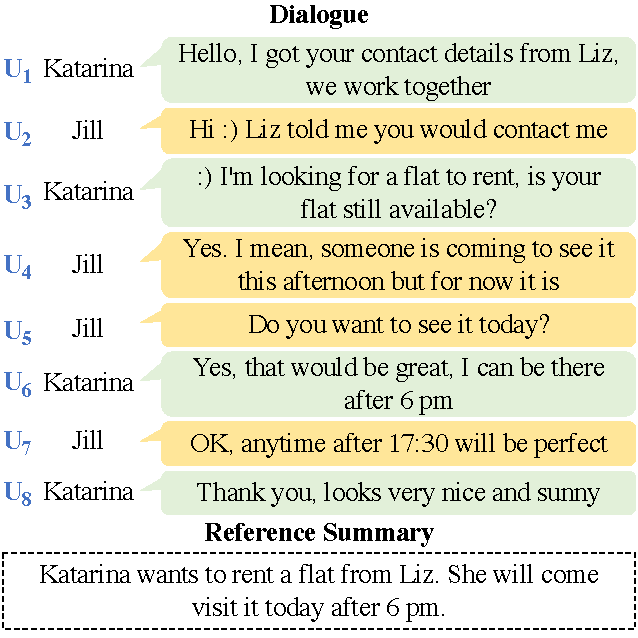
\includegraphics[scale=0.5]{fig/example.pdf}
	\caption{An example multi-party dialogue and its summary. The arrows represent unsequential dependencies between utterances. Elliptical sentences are in italic.}
	\label{fig:example}
\end{figure}

\textbf{Word Level - Language Style and Format:} 
Documents in previous well-researched summarization tasks are written from the third point of view, while dialogues consist of utterances expressed by different speakers in first person. Informal and colloquial expressions are common especially for recorded dialogues from speech, such as ``Whoa'' in $U_6$ and ``u'' representing ``you'' in $U_7$ from Figure~\ref{fig:example}.
Pronouns are frequently used to refer to events or persons mentioned in the dialogue history. Around 72\% of mentions in the conversation are {anaphoras} %pronouns
as stated in \citet{bai2021joint}. Meanwhile, the performance of coreference resolution models trained on normal text drops dramatically on dialogues~\cite{liu2021coreference}. It manifests the existence of language style differences between documents and dialogues, leading to difficulties in understanding the mappings between speakers and events in dialogues.


\textbf{Sentence/Utterance Level - Information Density:}
Document sentences are more self-contained with complete SVO (subject-verb-object) structures, while elliptical utterances are ubiquitous in dialogues, including $U_3$, $U_6$, $U_7$, $U_{11}$ and $U_{12}$.
Besides, the long dialogue can be summarized into a single summary sentence for the example in Figure~\ref{fig:example} as a result of back-and-forth questions and confirmations among speakers for communication purposes.
Question answerings, acknowledgments, and comments~\cite{asher2016discourse} are frequent discourse relations among utterances to narrow down speakers' information gaps and reach agreements.
In this way, dialogue utterances are highly content-dependent, and the information is scattered~\cite{zhang2021exploratory}, raising the difficulties for generating integral contents.

\textbf{Inter-sentence/utterance Level - Discourse structure:}
Articles tend to be well-structured, such as 
general-to-specific structure or deductive order. 
For example, the most important information 
in news summarization are always at the beginning of the document, resulting in a competitive performance of the simple Lead-$3$ baseline~\cite{nallapati2017, see2017get}. However, it is not the same for dialogue summarization. Both Lead-$3$ and Longest-$3$, i.e. $\{U1, U2, U3\}$ and $\{U4, U8, U9\}$ in Figure~\ref{fig:example}, get poor results in different dialogue scenarios~\cite{gliwa2019samsum,chen2021dialsumm,zhang2021emailsum}.
The dependencies among utterances are interleaved, shown by arrows in Figure~\ref{fig:example}, and discourse relations in dialogues are more flexible,
even with the correction of wrong information~\cite{asher2016discourse}. 
For example, 
Jake refused to be available for the reunion in $U_6$, but later agreed
in $U_8$.  As a result, it is more challenging to reason cross utterances for 
dialogue summarization than document summarization.

\textbf{Passage/Session Level - Topic boundaries:} Sentences under the same topic in documents are collected together in a paragraph or a section.
Previous works for extractive~\cite{xiao2019extractive} and abstractive summarization~\cite{cohan2018discourse} both took advantage of such features and made great progress. 
However, a dialogue is a stream of continuous 
utterances without boundaries, even for hours of discussion. The same topic may be discussed repeatedly 
with redundancies and new information, setting up obstacles for content 
selection in dialogue summarization.

%\JQ{it will be good to see the advantages of abstractive vs extractive approaches for dialogue summarization.}
%\JQ{add a little more about extractive methods, and explain why abstractive is more preferred especially in the case of dialogues.}
To better explain why abstractive approaches are more preferred than extractive ones for dialogues, we list the result of the best rule-based extractive baseline, i.e., Longest-$3$~\cite{gliwa2019samsum}, the oracle extractive result determined by Rouge-L Recall score between each summary sentence and dialogue utterances~\cite{chen2018fast}, and the generation by BART fine-tuned on SAMSum dataset~\cite{gliwa2019samsum} of the simple dialogue in Figure~\ref{fig:example} as follows:
\\
\begin{tabular}{|p{1.5cm}|p{\linewidth-2.3cm}|}
	\hline
	\textbf{Longest-$3$} & Jessica: If I move some things around, I can too! Jake: Hell yeah man! You know I freelance, worst case scenario I'll work from wherever we are Jessica: We should meet up where we did last time, it's perfect middle for everyone.\\
	\hline
	\textbf{Oracle} & Jake: Hell yeah man! You know I freelance, worst case scenario I'll work from wherever we are\\
	\hline
	\textbf{BART}& Ted, Pia, Jessica and Jake are going to meet up on Friday night. \\
	\hline
\end{tabular}
\\
We can see that the readability of generated summaries are poor for Longest-$3$ and Oracle due to the language style and format difference. The compression ratio of Longest-$3$ is apparently low while it still misses the involvement of Ted and Pia as a result of low information density of dialogues. Oracle is concise but much more information is missing. Meanwhile, the fine-tuned BART as an abstractive approach shows the favorable performance. Therefore, abstractive approaches becomes the mainstream in researches on dialogue summarization. In a word, dialogue summarization is an valuable research direction in summarization, where the modeling and understanding of dialogues are challenging compared with document summarization and abstractive approaches are especially preferred.
% despite some extractive summarization works~\cite{uma2022comparing,kano2020identifying,bokaei2016extractive}.
%@article{uma2022comparing,
%	title={Comparing Methods for Extractive Summarization of Call Centre Dialogue},
%	author={Uma, Alexandra N and Sityaev, Dmitry},
%	journal={arXiv preprint arXiv:2209.02472},
%	year={2022}
%}

%@inproceedings{kano2020identifying,
%	title={Identifying implicit quotes for unsupervised extractive summarization of conversations},
%	author={Kano, Ryuji and Miura, Yasuhide and Taniguchi, Tomoki and Ohkuma, Tomoko},
%	booktitle={Proceedings of the 1st Conference of the Asia-Pacific Chapter of the Association for Computational Linguistics and the 10th International Joint Conference on Natural Language Processing},
%	pages={291--302},
%	year={2020}
%}

%@article{bokaei2016extractive,
%	title={Extractive summarization of multi-party meetings through discourse segmentation},
%	author={Bokaei, Mohammad Hadi and Sameti, Hossein and Liu, Yang},
%	journal={Natural Language Engineering},
%	volume={22},
%	number={1},
%	pages={41--72},
%	year={2016},
%	publisher={Cambridge University Press}
%}


\subsection{Scenarios for Dialogue Summarization}\label{sec:scenarios}

Considering the source of dialogues and the purpose of doing summarization,
%\KZ{Rephrase this: dialogue sources and summary intentions}, 
we divide the application scenarios into two classes: \textbf{open-domain dialogue summarization (ODS)} and \textbf{task-oriented dialogue summarization (TDS)}. This taxonomy is similar to the one of dialogue systems~\cite{gao2020standard,chen2017survey}.
However, one should note that a pre-defined domain ontology for dialogues is 
not necessarily required for TDS, which is different from that in 
task-oriented dialogue systems.
The application scenarios investigated in previous papers 
are classified into these two classes as shown in Figure~\ref{fig:scenario}.

%\JQ{add citations}
Open-domain dialogue summarization is further divided into daily chat, 
drama conversation, debate \& comment. 
\textbf{Daily chat}~\cite{gliwa2019samsum,chen2021dialsumm} refers to the dialogues happening in our daily lives, 
such as making appointments, discussions between friends, etc. 
\textbf{Drama conversation}~\cite{rameshkumar2020storytelling,zhu2021mediasum,malykh2020sumtitles,chen2021summscreen} represents dialogues from soap operas, 
movies or TV shows, which are dramatized or fabricated with drama scripts 
behind them. Dialogues in these two classes are full of person names 
and events, resulting in narrative summaries about ``who did what''.
\textbf{Debate \& comment}~\cite{misra2015using,fabbri2021convosumm,chowdhury2019cqasumm} focuses more on question answering and 
discussions in online forums and arguments. These dialogues emphasize opinions or solutions to the given subject or questions.

Task-oriented dialogue summarization arises from application scenarios of different domains, which includes but is not limited to customer service, 
law, medical care and official issue.
\textbf{Customer service}~\cite{zou2021topic,feigenblat-etal-2021-tweetsumm-dialog,zhao2021todsum,liu2019automatic,chen2020jddc} refers to conversations between customers and service providers.
Customers start the conversation with their specific intents and agents are required to meet these requirements with the help of their in-domain databases, such as hotel reservations and express information consultation for online shopping. Dialogue summarization for this task is mainly to help service providers quickly go through solutions to users' questions for agent training and service evaluation. 
\textbf{Law}~\cite{fuzw20,duan2019legal,xi2020global} is dialogues related to legal service and 
criminal investigations. Dialogue summarization in this scenario alleviates the recording and summarizing workload 
for law enforcement or legal professionals. 
\textbf{Medical care}~\cite{joshi2020dr,song2020summarizing,song2020summarizing,zhang2021leveraging,liu2019topic} is dialogues between doctors and patients and medical dialogue summarization has some similarity to the research on electronic health records (EHR). Unlike the previous work focusing on mining useful information from EHR~\cite{yadav2018mining}, summarization is to extract useful information from the doctor-patient dialogue and generate an EHR-like or fluent summary for clinical decision-making or online search. It also aims to reduce the burden of domain experts.
\textbf{Official affair}~\cite{carletta2005ami,janin2003icsi,ulrich2008publicly,zhang2021emailsum} is conversations between colleagues for technical or teachers and students for academic issue discussion. They can be either in the format of meetings or e-mails, with summaries covering problems, solutions, and plans.


\begin{figure}
	\centering
	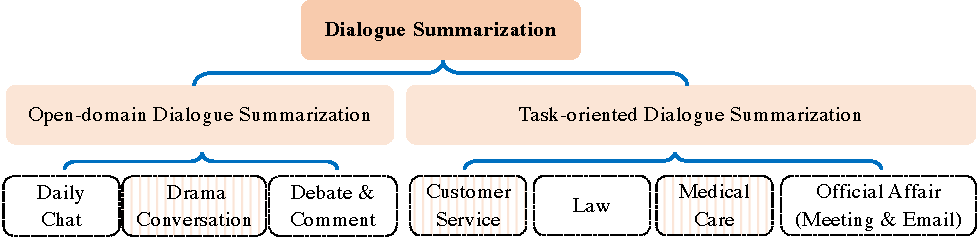
\includegraphics[scale=0.8]{fig/scenarios.pdf}
	\caption{The classification of dialogue summarization tasks with different application scenarios. Datasets proposed for evaluations under each scenario are in Section~\ref{sec:dataset}.}
	\label{fig:scenario}
\end{figure}


We compare and contrast ODS and TDS as follows.
\begin{itemize}
% functional role playing
\item Dialogues happen between \textbf{two or more speakers} both in ODS and TDS, whereas the \textbf{interpersonal relationship} and \textbf{functional relationship} among speakers are different. Generally, speakers in ODS are friends, neighbors, lovers, family members, and so on. 
They are equal either in the aspect of interpersonal relationships or functional relationships. For example, one can raise a question or answer others' questions in online forums~\cite{fabbri2021convosumm}.
In TDS, speakers have different official roles acting for corresponding responsibilities. For example, plaintiff, defendant, witness and judge in court debates~\cite{duan2019legal}, project manager, marketing expert, user interface designer and industrial designer in official meetings~\cite{carletta2005ami} are corresponding roles.
Among different dialogues, roles are the same and can be played by different speakers and a speaker's role is always unchanged for a service platform.
In a word, TDS pays more attention to functional roles while ODS focuses on speakers.


% covering topics
\item Multiple \textbf{topics} may be covered in the same dialogue session.
Topics in ODS are more diverse than in TDS. The summarization models are expected to deal with unlimited open-domain topics such as chitchat, sales, education, and climate at the same time~\cite{chen2021dialsumm}. 
However, topics in TDS are more concentrated and need more expertise for understanding.
Dialogues in TDS either focus on a single domain with more fine-grained topics, such as medical dialogues of different specialties,
or several pre-defined domains, such as restaurant, hotel, and transformation reservation.
Domain knowledge is significant for summarization, and it is divergent across sub-domains. For instance, expertise and medical knowledge are required in doctor-patient dialogues for generating accurate medical concepts~\cite{joshi2020dr} while specific knowledge bases for internal medicine and primary care are not the same.

%  inherent structure
\item The input dialogue for both ODS and TDS is made up of \textbf{a stream of utterance} as defined in Equation~\ref{eq:dialogue}. However, 
the \textbf{structure} of these two types of dialogues are different.
Open-domain dialogues often happen casually and freely while dialogues in TDS may have some inherent working procedures or writing formats. 
For example, the program manager in meetings usually masters the meeting progress~\cite{zhu2020end} implicitly with words such as ``okay, what about ...'', and communications by e-mails consist of semi-structured format including subjects, receivers, senders, and contents~\cite{zhang2021emailsum}. 

% special intentions for summaries
\item \textbf{Focuses of summaries} are distinct. Summaries for ODS in recent research are more like condensed narrative paraphrasing with different levels of granularity. An example is a synopsis from the Fandom wiki\footnote{\url{criticalrole.fandom.com}} maintained by fans for the Critical Role transcripts~\footnote{\url{github.com/RevanthRameshkumar/CRD3}}\cite{rameshkumar2020storytelling}, helping to quickly catch up with what is going on in the long and verbose dialogues. Differently, dialogues in TDS take place with strong intentions for solving problems. Summaries for such dialogues are expected to cover the user intents and corresponding solutions, such as medical summaries for clinical decision making~\cite{joshi2020dr} and customer service summaries for ticket booking~\cite{zhao2021todsum}. As a result, generating faithful content is extremely significant for TDS. %{faithfulness}
\end{itemize}

%\KZ{I feel that just dividing the dialogue summarization into ODS and TDS is a bit
%too coarse-grained. Later when you discuss the approaches, u need to associate
%each approaches with a certain characteristic/scenario of the task. It's more
%useful if u can use some refined characteristics of the task.}

\section{Background and Related Work}
In this section, we present the necessary background knowledge about matrix factorization and unstructured pruning (\figref{fig:intro}).

\begin{figure}[t!]
	\centering
	\scalebox{0.154}{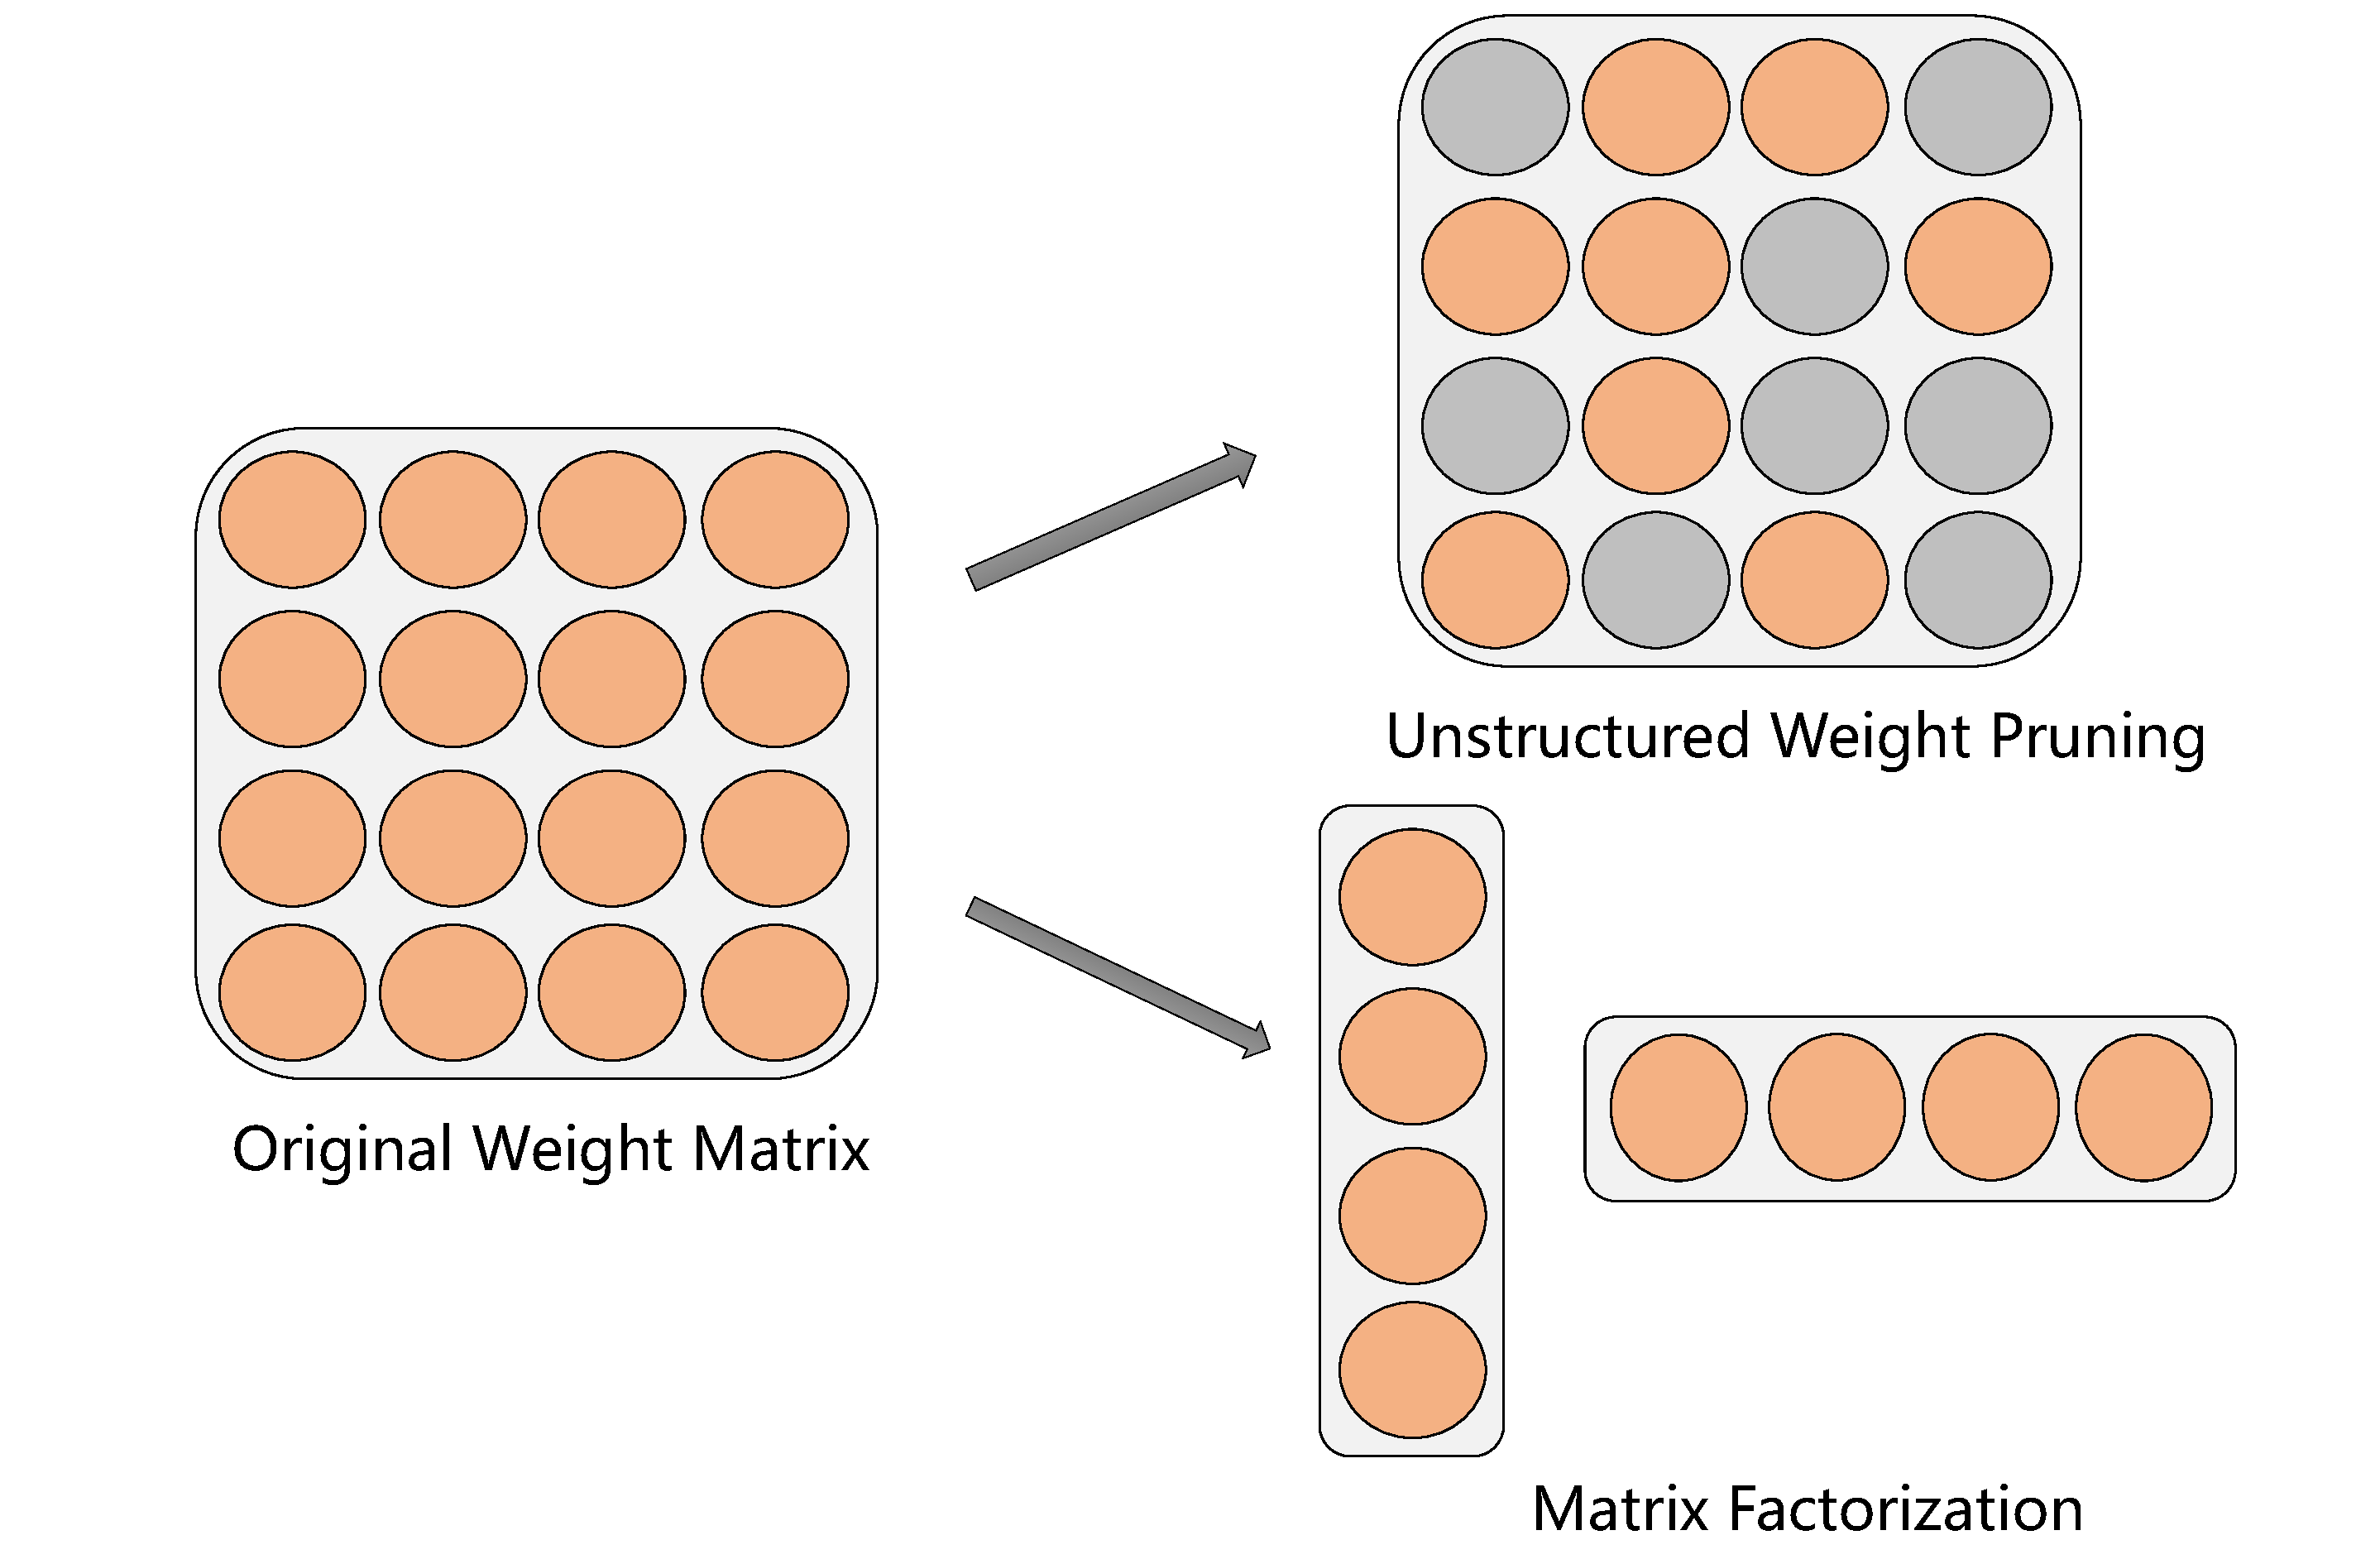
\includegraphics{./figures/intro_final.pdf}}
	\caption{Illustration of matrix factorization and unstructured pruning  on a single weight matrix.}
	\label{fig:intro}
\end{figure}

\subsection{Matrix Factorization~(MF)}
\label{sec:lr}
Given the weight matrix $\bm{W}\in \mathbb{R}^{n\times m}$, matrix factorization~\cite{svd} decomposes it into sub-matrices with reduced total number of parameters to achieve model compression.  
It first uses singular value decomposition~(SVD) to obtain an equivalent 
form of $\bm{W}$ as the product of three matrices:
\begin{align}
	\bm{W}=\bm{U}\bm{\Sigma}\bm{V}^\mathrm{T}
\end{align}
where $\bm{U}\in \mathbb{R}^{n\times r}$, $\bm{\Sigma}\in  \mathbb{R}^{r\times r}$, $\bm{V}\in \mathbb{R}^{r\times m}$, and $r$ is the rank of matrix $\bm{W}$. $\bm{\Sigma}$ is a diagonal matrix of non-zero singular values $\{\sigma_1, \sigma_2,...,\sigma_r\}$ in descending order. Then, low-rank approximation with targeted rank $k$ is obtained by keeping the top-$k$ singular values in $\bm{\Sigma}$ as well as their corresponding column vectors in $\bm{U}$ and $\bm{V}$:
\begin{align}
	\bm{W}&\approx \bm{U}_{[:, :k]}\bm{\Sigma}_{[:k,:k]}\bm{V}_{[:, :k]}^{\mathrm{T}} =\bm{A}\bm{B}
	\label{eq:svd}
\end{align}
where $\bm{A}=\bm{U}_{[:,:k]}\bm{\Sigma}_{[:k,:k]}$ and $\bm{B}=\bm{V}_{[:,:k]}^{\mathrm{T}}$ are the two final sub-matrices of which the product is used to replace $\bm{W}$. After such factorization, the number of parameters is reduced from $nm$ to $k(n+m)$. Different compression rates can be achieved by varying the preserved rank $k$.



\subsection{Unstructured  Pruning~(UP)}
\label{sec:pruning}
%We first establish some shared notations for unstructured weight pruning. 
Let $\bm{W}\in \mathbb{R}^{n\times m}$ denote a generic weight matrix in a PLM. In order to determine which elements in $\bm{W}$ are pruned, an importance score matrix $\bm{S}\in \mathbb{R}^{n\times m}$ is correspondingly introduced. The smaller $S_{i,j}$ is, the larger the probability of $W_{i,j}$ will be pruned. Given the importance scores, a pruning strategy $f_{prune}(\cdot)$ computes a binary mask matrix $\bm{M}\in \{0,1\}^{n\times m}=f_{prune}(\bm{S})$, 
and the forward process for an input $x$ becomes $y=(\bm{W}\odot\bm{M})x$, 
where $\odot$ denotes element-wise multiplication.

\paragraph{Zero-order Pruning~(UP$_{\text{zero}}$)} Zero-order pruning refers to the family of algorithms that only use the value of the weight as the importance measure.
For example, magnitude-based weights pruning~\cite{mag,chen2020lottery} adopts the absolute value of weight as importance score, i.e., 
$\bm{S}_{i, j}=|\bm{W}_{i, j}|$. The typical choice of $f_{prune}(\cdot)$ is to keep $v\%$  of weights with the largest importance scores:
\begin{align}
	\bm{M}_{i,j}=
	\begin{cases} 
		1, & \text{if }\bm{S}_{i,j}~\text{is in the largest }v\%\\
		0,  & \text{otherwise}  
	\end{cases}
	\label{eq:zero}
\end{align}


\paragraph{First-order Pruning~(UP$_\text{first}$)} Unlike zero-order pruning where $\bm{S}$ is directly derived from $\bm{W}$, first-order methods treat 
$\bm{S}$ as learnable parameters and jointly train it with model weights 
during fine-tuning. For example, SMvP~\cite{movement} and CAP~\cite{cap}
randomly initialize $\bm{S}$ and update it during the whole pruning process. The pruning strategy $f_{prune}(\cdot)$ is the same as in zero-order pruning~(\eqnref{eq:zero}).


%\begin{align}
%	\bm{M}_{i,j}=
%	\begin{cases} 
%		1, & \text{if }\bm{S}_{i,j}\ge \tau\\
%		0,  & \text{otherwise}  
%	\end{cases}
%	\label{eq:first}
%\end{align}
Since the gradient of the thresholding function is 0 everywhere, straight-through estimator~\cite{st} is used as an approximation. The importance score $\bm{S}_{i,j}$ of $\bm{W}_{i,j}$ up to training step $T$ can be expressed as: 
\begin{align}
\bm{S}_{i,j}=-\sum_{t\le T}(\frac{\partial \mathcal{L}}{\partial \bm{W}_{i,j}})^{(t)} \bm{W}_{i,j}^{(t)}
\end{align}
where $\mathcal{L}$ is the loss function. The formulation is also equivalent to the first-order Taylor approximation of the change in $\mathcal{L}$ if $\bm{W}_{i,j}$ is zeroed out.

\paragraph{Sparsity Scheduler}
The proportion of remaining weights is controlled by the sparsity scheduler, here  we adopt the commonly used  cubic sparsity schedule to progressively reach target sparsity, i.e., $v_t$ at time step $t$ is derived by:
\begin{align}
	%	v^{(t)}=
	\begin{cases} 
		v_i & t\in [0, t_i) \\
		v_f+(v_i-v_f)(\frac{T-t_{f}-t}{T-t_f-t_i})^3 & t\in[t_i, T-t_f) \\
		v_f  & \text{otherwise}  
	\end{cases}
\end{align}
\label{eq:prune}
where $v_i=1.0$, $v_f$ is the final percent of remained parameters, $t_i$ and $t_f$ are the warmup and cool-down steps. $T$ is the total training steps. Moreover, we discard $\bm{M}$ and directly set $\bm{W}_{i,j}$ to zero if $\bm{S}_{i,j}^{(t)}$ is not in the top-$v_t$ at time step $t$. 
%\paragraph{A Unified View} The differences in the implementation of 
%importance scores~(direct value inspection v.s. additional learnable 
%parameters) and pruning strategy~(top-$v$ selection v.s. tuned threshold) 
%make it hard to compare various pruning methods. To this end, 
%we establish a unified view of zero-order and first-order pruning, 
%denoted as \textbf{UWP$_\text{zero}$} and \textbf{UWP$_\text{first}$}, 
%with the only difference being the calculation of importance score $\bm{S}$.
%\KZ{This section is a little strange here because it seems to repeat
%what has been said in the previous subsections. You have already defined $S$
%but now you are singling out $S$ again. In particular, I can't appreciate why
%``it is hard to compare various pruning methods'', I don't really see
%the need for this unified view.}
%
%For UWP$_\text{zero}$, the calculation of $\bm{S}$ is the same as magnitude pruning, i.e., $\bm{S}_{i, j}^{(t)}=|\bm{W}_{i, j}^{(t)}|$, where $t$ is the time step. For UWP$_\text{first}$, we directly calculate its importance score $\bm{S}$ without introducing additional parameters, i.e.,  $\bm{S}_{i,j}^{(t)}=\bm{S}_{i,j}^{(t-1)}+|\frac{\partial \mathcal{L}}{\partial \bm{W}_{i,j}}^{(t)} \bm{W}_{i,j}^{(t)}|$. 

%\KZ{\eqref{eq:prune} seems 
%to be something new in this section but then it is part of the first-order 
%pruning, and nothing to do with zero-order pruning. So why is it in the 
%``unified view?''}

%\KZ{My feel is that this whole section of related work and background is a bit
%long-winded.}
 


\section{Preliminary Study}
\label{sec:pilot}
In this section, we conduct a preliminary study on unstructured pruning  and matrix factorization
based on BERT-base and try to find answers to the following two questions: (1) How does matrix factorization perform under high compression rates? (2) Do subnetworks produced by unstructured pruning contain \textit{low-rank} sparsity patterns while preserving the majority of task accuracy?
%\KZ{What kind of insight? You stop short of providing the motivation
%of the following experiments. Are you trying to see if these two methods alone
%work well to compress language model?}

\subsection{Experimental Setting}
\indent
\paragraph{Datasets}We use two tasks from GLUE benchmark~\cite{glue}, namely MRPC and RTE, as our evaluation testbeds. Both of them are formulated as classification problems.

\paragraph{Implementation Details} For matrix factorization, we follow the algorithm in \secref{sec:lr}. Specifically, we first fine-tune BERT-base on each downstream task following \citet{bert}. Then, we perform truncated SVD on weight matrices of each linear layer in the fine-tuned BERT and re-train the whole model to recover the lost accuracy. We select preserved rank $k$ from $\{390, 260, 130, 50\}$, which corresponds to $\{0.75, 0.50, 0.25, 0.10\}$ of BERT's parameters.

For unstructured  pruning, we evaluate both UP$_\text{zero}$ and UP$_\text{first}$. We set the value of $v_f$ from $\{0.75, 0.50, 0.25, 0.10\}$ to make a direct comparison to matrix factorization.

\subsection{Results and Analysis}
\label{sec:pilot_results}

%\begin{figure*}[t]
%	\centering
%	\scalebox{0.285}{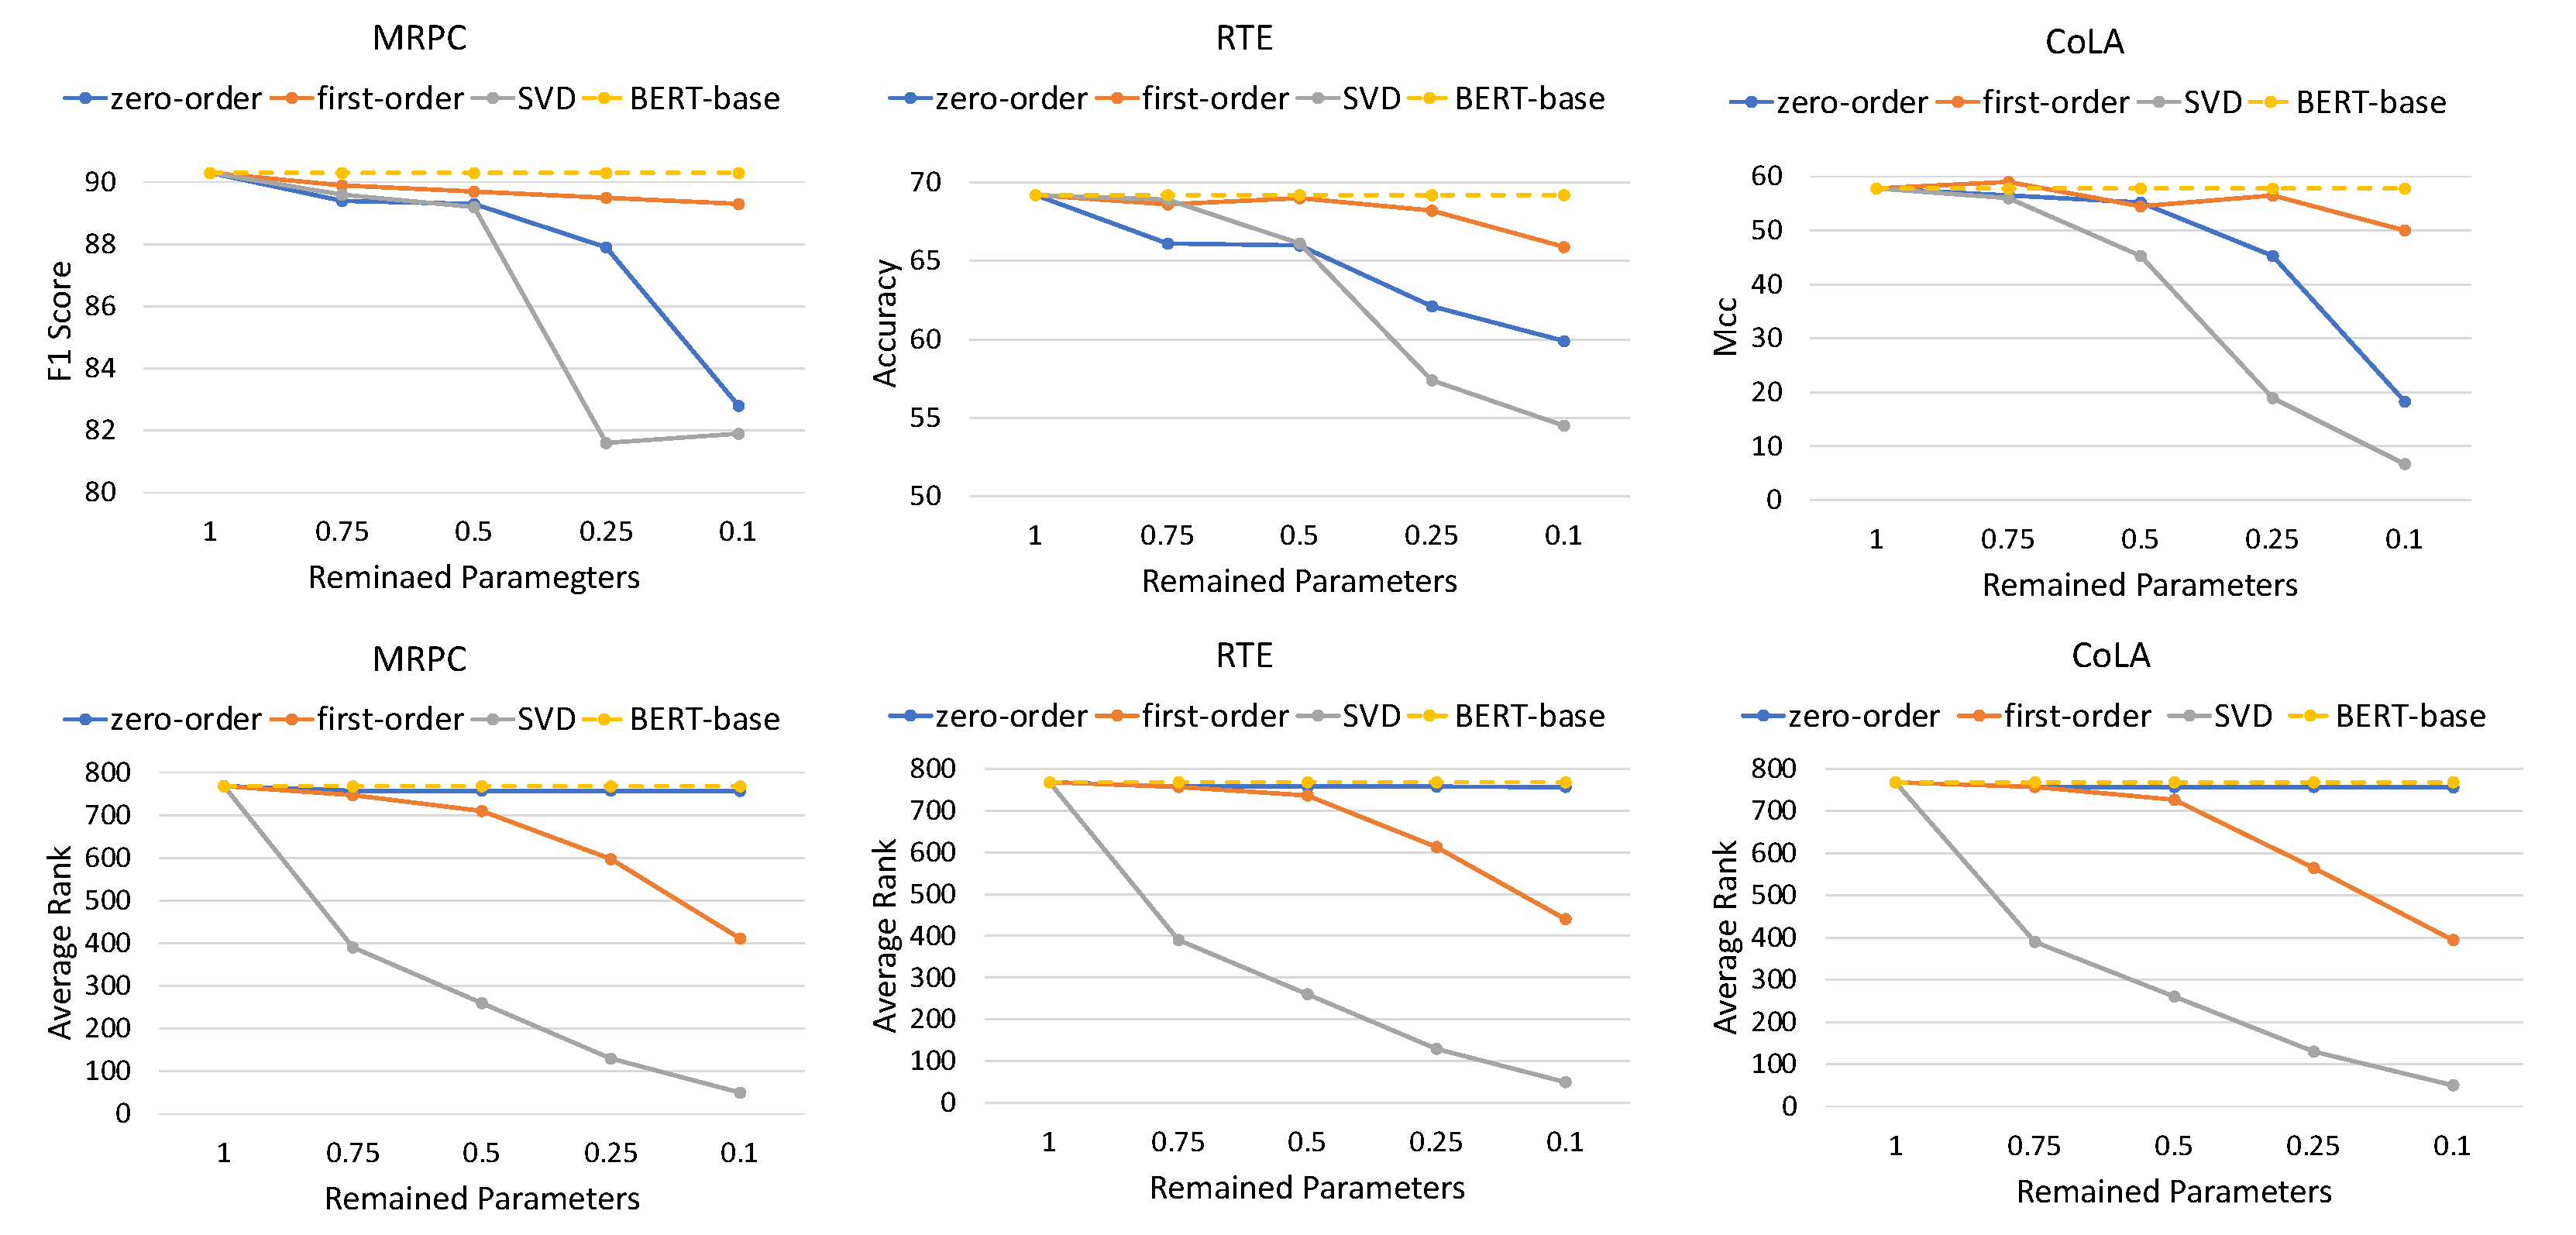
\includegraphics{./figures/pre_new.pdf}}
%	\caption{Task performance~(top half) and average matrix rank~(bottom half) v.s. percent of remained parameters. The dashed yellow line indicates the performance/rank upper bound by fine-tuning the full-scale BERT-base model.}
%	\label{fig:pre}
%\end{figure*}


\paragraph{Accuracy Preservation} 
The variation of task accuracy with respect to the remaining parameters is illustrated 
in the top half of \figref{fig:pre}. Under a small compression rate, i.e., 
$75\%$  parameters remaining, all examined methods can retain $\ge 97\%$ performance 
of BERT-base across all tasks. Under moderate compression rate, i.e., $50\%$ parameters remaining, UP$_\text{zero}$ and SVD start to show obvious declines. 
When more extreme compression rates are pursued, e.g., $25\%$-$10\%$ parameters 
remaining, SVD exhibits the most drastic performance drops compared to UP methods. 
On the contrary,  UP$_\text{first}$ still retains $\sim 97.6\%$ of BERT's performance.
UP$_\text{zero}$ lags behind UP$_\text{first}$ by a large margin under high sparsity. This indicates that magnitude alone cannot be used to quantify a weight's 
contribution because even a small weight can yield a huge influence on the model 
output due to the complicated compositional nature of neural networks. 
In contrast, the importance criterion of UP$_\text{first}$ directly reflects the 
sensitivity of the model's training loss w.r.t. each weight and is therefore more 
accurate.

\begin{figure}[t]
	\centering
	\scalebox{0.175}{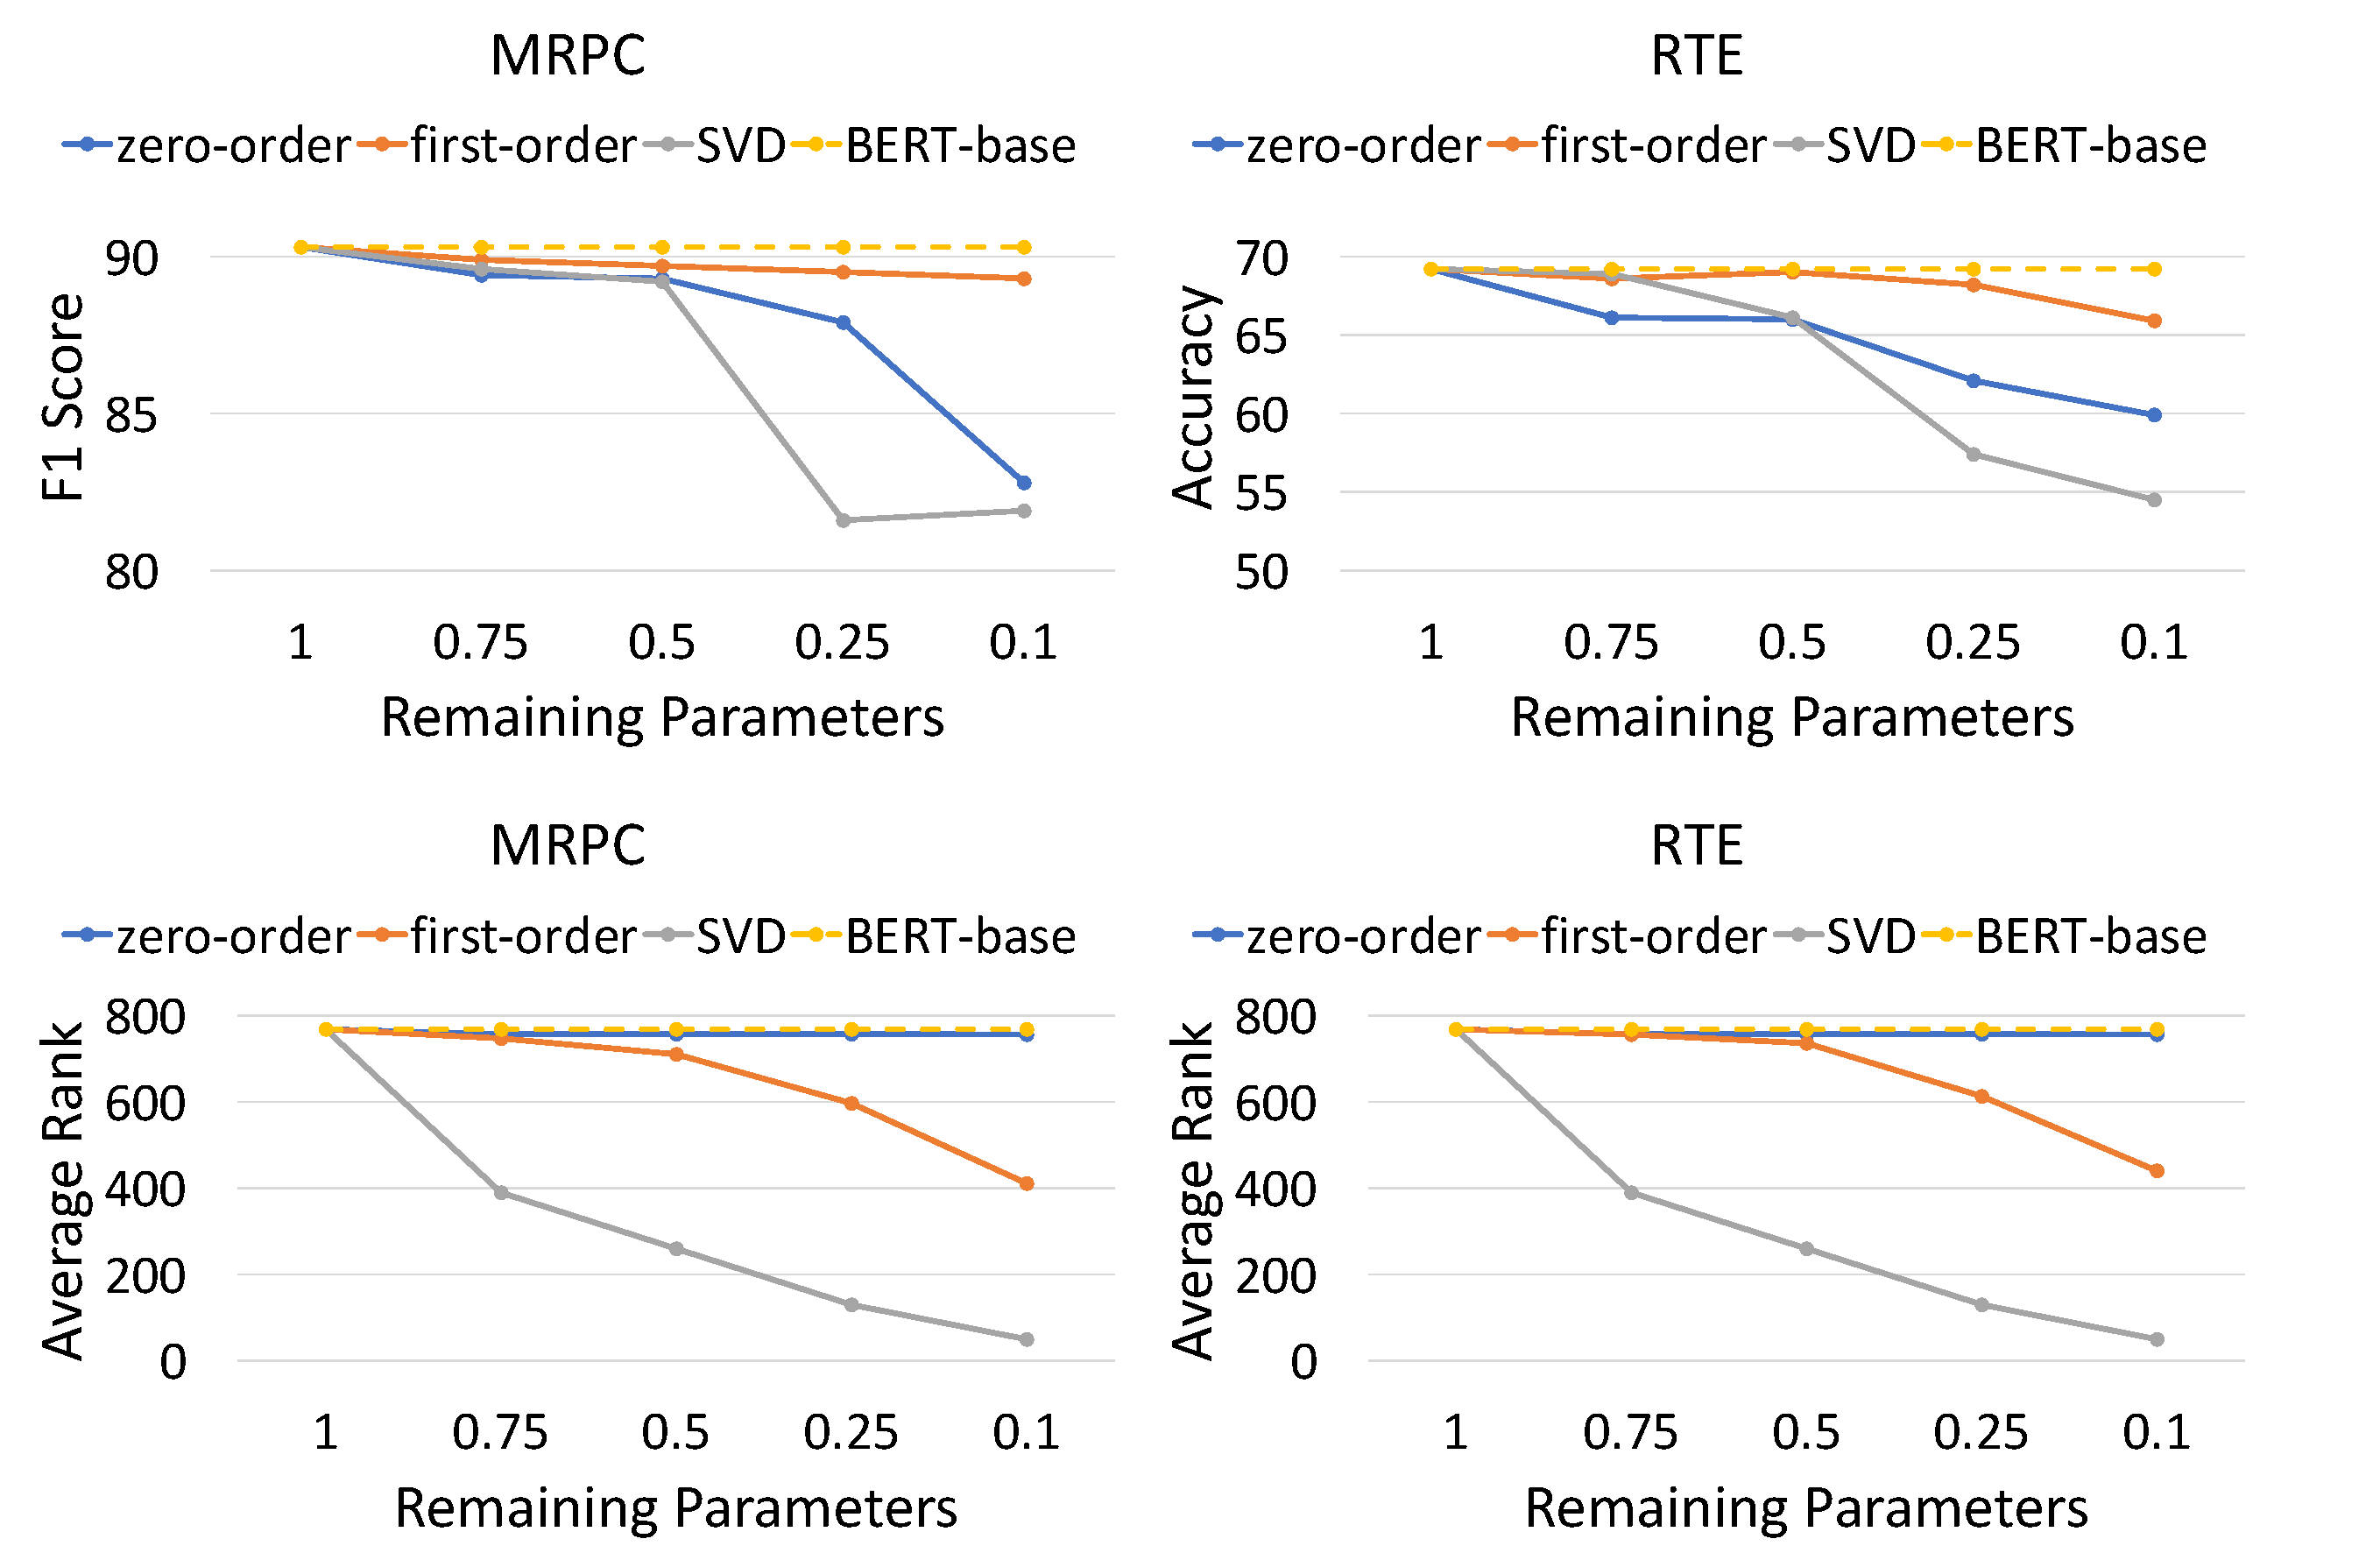
\includegraphics{./figures/pre_col.pdf}}
	\caption{Task accuracy~(top half) and average matrix rank~(bottom half) 
v.s. percentage of original parameters retained. 
The dashed line indicates the performance/rank upper bound by fine-tuning the full-scale BERT-base model. Results on more datasets are deferred to Appendix \ref{sec:A}.}
	\label{fig:pre}
\end{figure}

\begin{figure}[t]
	\centering
%	\scalebox{0.50}{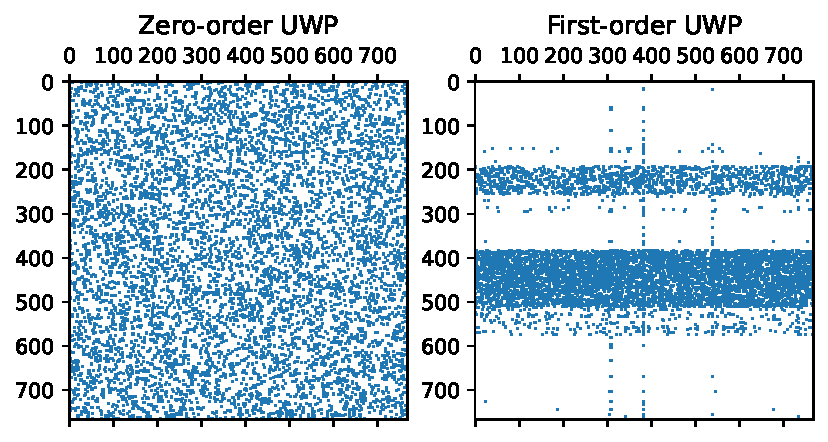
\includegraphics{./figures/sparsity_pattern.pdf}}
		\scalebox{0.50}{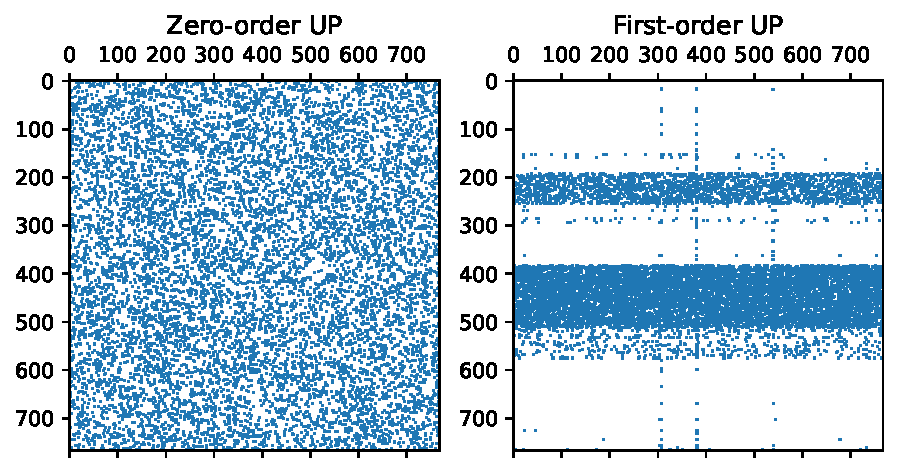
\includegraphics{./figures/zero_first_UP.pdf}}
	\caption{Sparsity patterns of the same 768x768 weight matrix  pruned by UP$_\text{zero}$~(left) and UP$_\text{first}$~(right) on MRPC with $10\%$ of
the parameters remaining.}
	\label{fig:pattern}
\end{figure}

\paragraph{Rank} 
Considering the inferior accuracy of SVD, we hypothesize that the weight matrices of fine-tuned BERT are high-rank, 
hence leading to a large approximation error when $k$ is small. The bottom half of \figref{fig:pre} inspects the average rank of weight matrices. We can see that the weight matrices in fine-tuned BERT-base are nearly full-rank, which explains the inefficacy of SVD when $k$ is small. We also plot the rank-parameter curve of UP methods. For UP$_\text{zero}$, it produces sparse matrices that are 
as high-rank as densely fine-tuned BERT even when $90\%$ weights are set to zero. In contrast, UP$_\text{first}$  produces sparse patterns whose rank monotonically decreases as more weights are pruned. To gain more insights into this phenomenon, we visualize the weight matrix pruned by UP$_\text{zero}$ and UP$_\text{first}$ in \figref{fig:pattern}. Though both are designed without structural bias,  unlike UP$_\text{zero}$, UP$_\text{first}$ learns to remove entire rows from the weight matrix and 
the resulting matrix enjoys a low-rank characteristic.



\begin{figure}[th]
	\centering
	\scalebox{0.142}{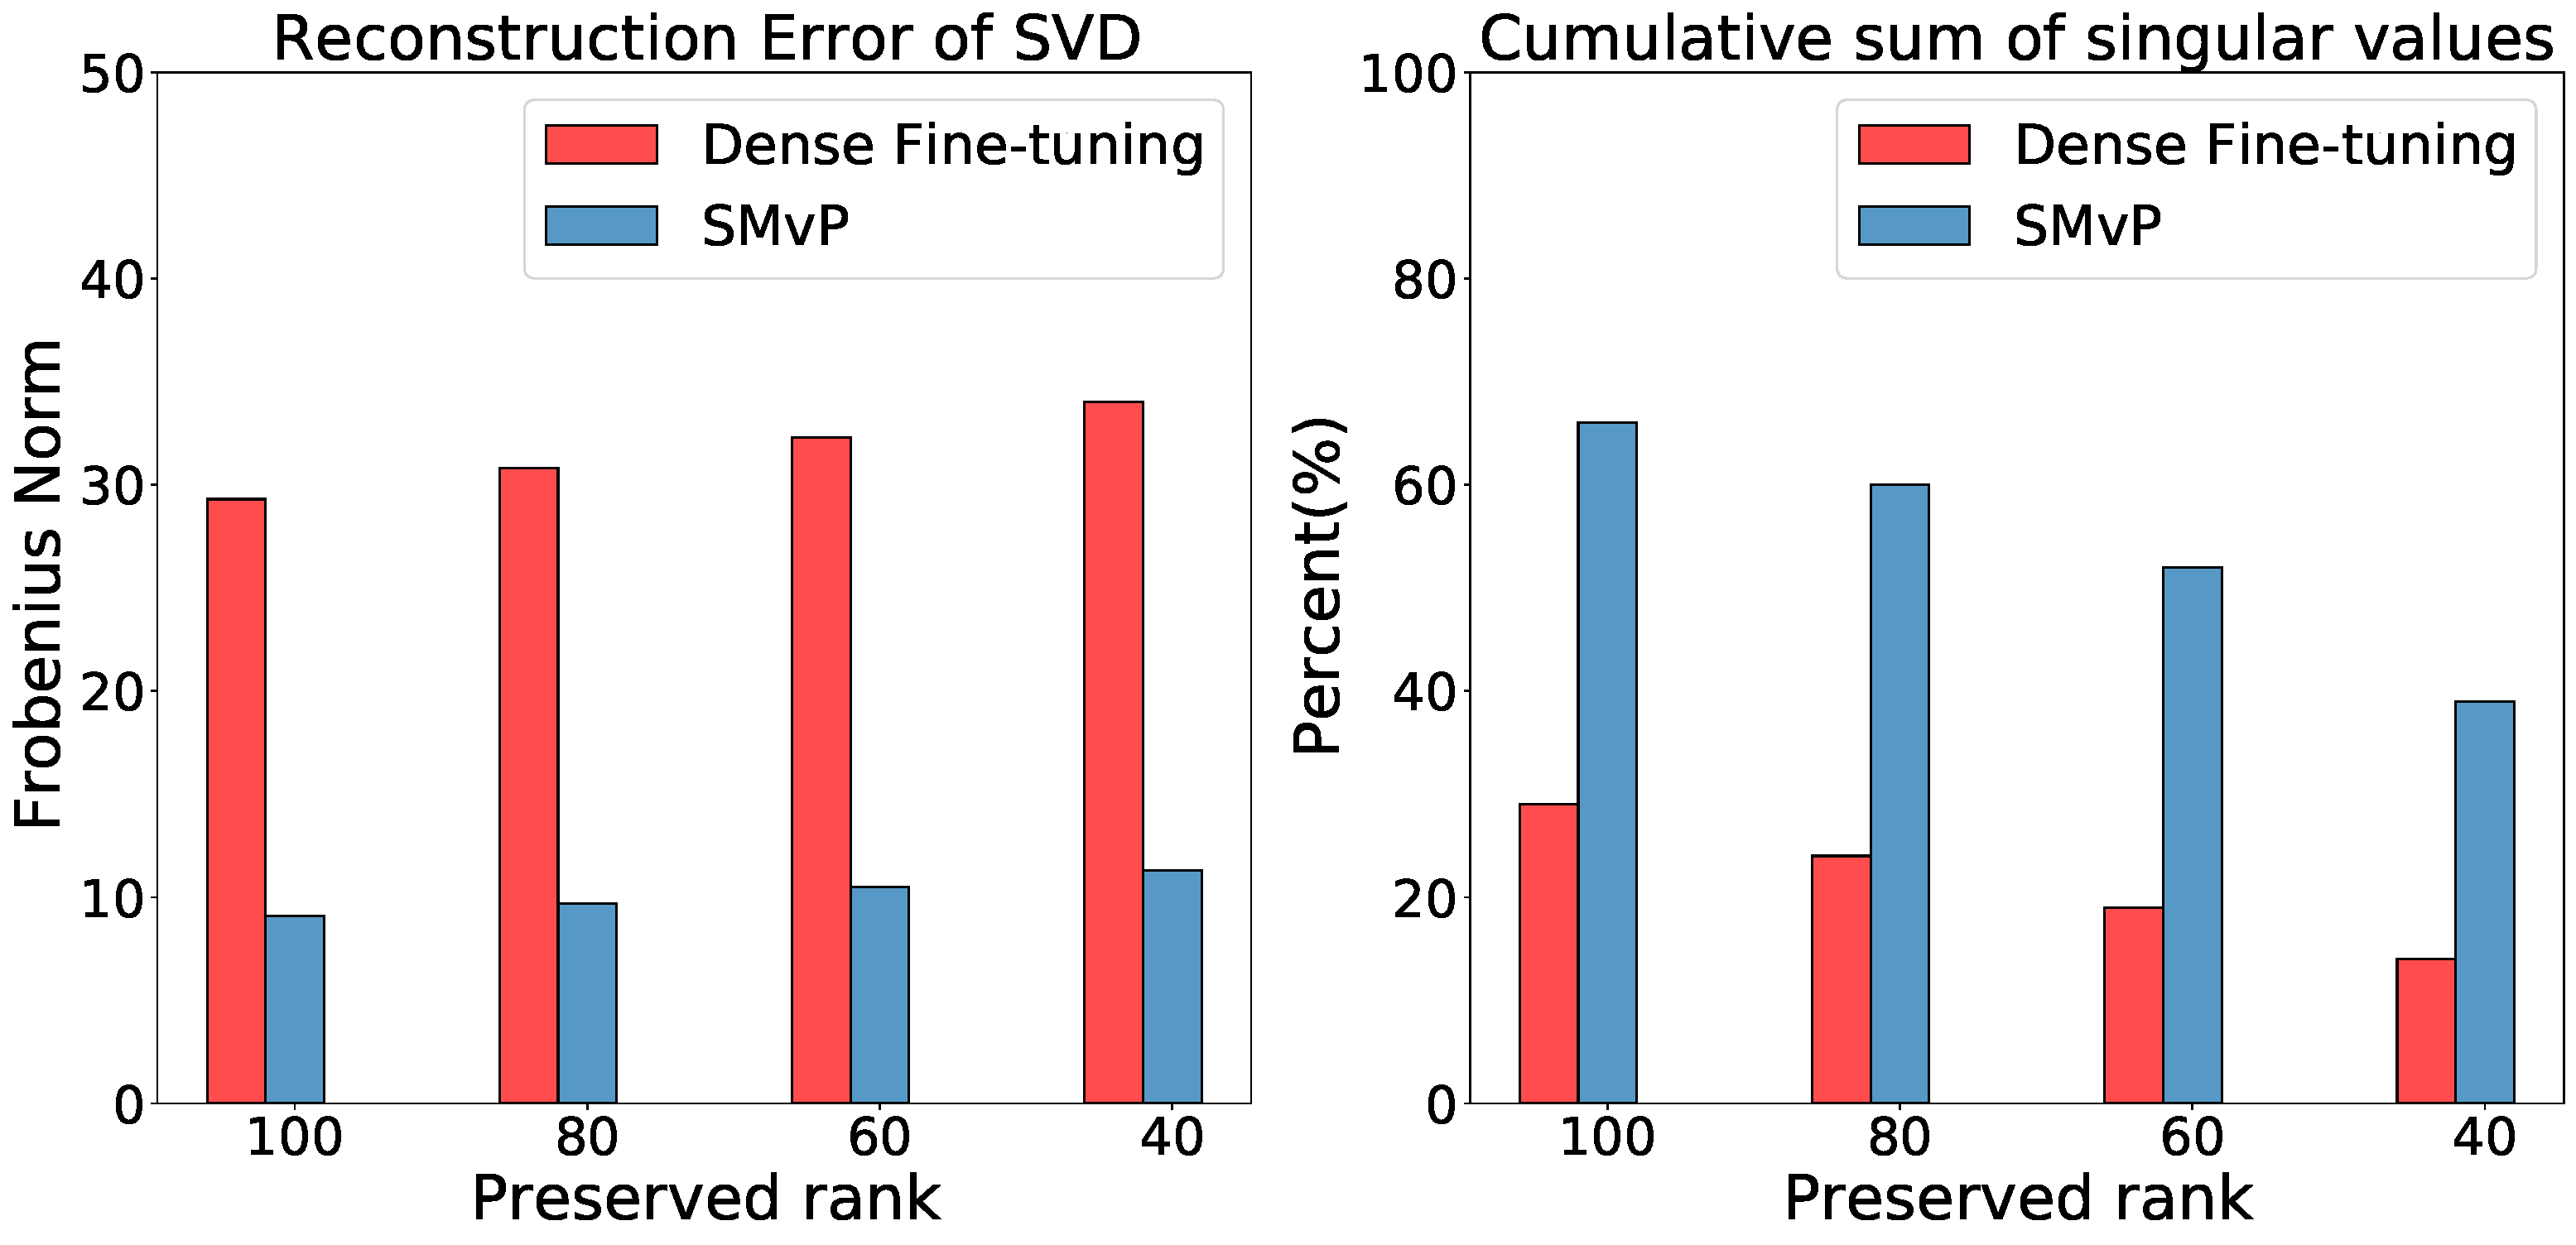
\includegraphics{./figures/norm_vis.pdf}}
	\caption{Quantitatively measuring approximation quality via reconstruction error~(left) and cumulative sum of singular values~(right) on MRPC.}
	\label{fig:norm}
\end{figure}

\paragraph{The Idea}
%\KZ{The key insight is: factorize a high-rank matrix into low rank sub-matrices
%loses a lot of info, but factorize a low-rank matrix into low rank sub-matrices
%doesn't lose as much info. Our design is based on this insight. I think as long
%as you make this insight clear, that's good enough. Some of this section
%is a bit verbose.} 
%Given the fact that factorizing from a low-rank matrix into sub-matrices loses less information than factorizing from a high-rank matrix
%Given the competitive task performance and low-rank structure of UWP$_\text{first}$, 
%it appears plausible to perform low-rank matrix factorization on 
%low-rank sparse models for model compression. 
The key insight is: factorizing a high-rank matrix into low rank sub-matrices
loses significant quantity of useful information, but factorizing a low-rank matrix into low rank sub-matrices
doesn't lose as much information. Our design is based on this insight. 
As a sanity check of its feasibility, we quantitatively measure the 
quality of low-rank approximation with various preserved ranks $k$. 
\figref{fig:norm} shows that given a specific $k$, 
the sum of top-$k$ singular values of matrices produced by UP$_\text{first}$ takes a much larger portion of total values than fine-tuning, suggesting that we can reserve more information of low-rank sparse matrix given the same $k$. The reconstruction error~(measured by Frobenius norm) of UP$_\text{first}$ is also significantly lower, implying a higher approximation quality. We thus expect that low-rank matrix factorization on low-rank sparse models to effectively combine: 
(1) the good performance of first-order UP; 
(2) direct memory and computation reduction by MF.

\section{LPAF: Low-rank Prune-And-Factorize}
\label{sec:approach}
Here we formally propose the LPAF~(\textbf{L}ow-rank \textbf{P}rune-\textbf{A}nd-\textbf{F}actorize) framework 
for language model compression. In addition, 
we propose two optimizations in the 
initialization and training of the compression process.

\subsection{The Overall Workflow}
\label{sec:ptf}
Given a pre-trained language model $T$ and a downstream task with training set $D=\{(x_i, y_i), i=1,2,...M\}$, LPAF consists of three steps to realize model compression: 
\begin{itemize}
	\item Step-1: obtaining the low-rank sparse model $T_{\text{sparse}}=\text{UP}_\text{first}(T,D, v)$. $v$ is the percent of remained parameters after pruning.
	\item Step-2:  performing matrix factorization on each weight matrix~(excluding the embedding layer) in $T_{\text{sparse}}$ and  obtain its low-rank factorized form $T_{\text{factorized}}$. 
	%	The perceivable reduction of model's memory footprint and computation cost happens at this step.
	\item Step-3:  re-training $T_{\text{factorized}}$ on $D$ using task-specific loss function until convergence. 
	%	Since step 2 inevitably loses certain task-specific information, this step is designed to ensure that the compressed model retain good task performance.
\end{itemize}

Next, we present two novel optimizations, namely \textit{sparsity-aware SVD} and \textit{mixed-rank fine-tuning}, that improves the matrix factorization and fine-tuning process in step 2 and step 3 respectively.

\subsection{Optimization 1: Sparsity-aware SVD}
\label{sec:sasvd}
SVD has been shown~\cite{bestsvd} to provide the optimal rank-$k$ approximation to $\bm{W}$ with respect to the Frobenius norm:
\begin{align}
	\nonumber
	\min_{\bm{A},\bm{B}} ||\bm{W}-&\bm{A}\bm{B}||_{F}=\min_{\bm{A},\bm{B}} \sum_{i,j}(\bm{W}_{i,j}-(\bm{AB})_{i,j})^2 \\
	& \text{s.t.}~~~~\text{rank}(\bm{AB})=k
\end{align}
It is a generic factorization method in that it is applicable to any matrix $\bm{W}$ by penalizing the reconstruction error of each individual weight equally. 

In our case, $\bm{W}$ is a sparse matrix from $T_{\text{sparse}}$ in which the majority of weights are set to zero by the pruning algorithm $P$. These zero weights are deemed to have less impact on the task performance compared to the retained~(unpruned) weights. However, the vanilla SVD treats each weight equally without considering the inherent sparseness of $W$, thus may be sub-optimal for preserving useful information in $W$ about the end task.
To address this issue, we propose sparsity-aware SVD which considers different priorities of parameters and weighs the individual reconstruction error based on its importance score $\bm{S}_{i,j}$:
\begin{align}
	\min_{\bm{A},\bm{B}} \sum_{i,j}&\bm{S}_{i,j}(\bm{W}_{i,j}-(\bm{AB})_{i,j})^2~~~\\\
	 & \text{s.t.}~~\text{rank}(\bm{AB})=k
	\label{eq:sasvd}
\end{align}
In this way, parameters that are more important can be better reconstructed, hence retaining more task performance from $T_{\text{sparse}}$ at initialization. Nevertheless, \eqnref{eq:sasvd} does not have a closed form solution~\cite{weightedsvd,hsu2021language} when each $\bm{W}_{i,j}$ has its own weight. We therefore resort to a simplification by letting the same row of $\bm{W}$ share the same importance. The importance for row $i$ is given by $\hat{\bm{S}}_{i}=\frac{\sum_{j}\bm{S}_{i,j}}{\sum_{n}\hat{\bm{S}}_{n}}$. Let $\hat{\bm{I}}=diag(\hat{\bm{S}}_1,\hat{\bm{S}}_2,...,\hat{\bm{S}}_{n})$ denote a diagonal matrix,  \eqnref{eq:sasvd} is now converted to:
\begin{align}
	&\min_{\bm{A},\bm{B}}||\hat{\bm{I}}\bm{W}-\hat{\bm{I}}\bm{A}\bm{B}||_F~~~~
	\\
	& \text{s.t.}~~\text{rank}(\bm{AB})=k
\end{align}
This essentially amounts to applying rank-$k$ SVD upon $\hat{\bm{I}}\bm{W}$, i.e., $\hat{\bm{I}}\bm{W}=\hat{\bm{U}}\hat{\bm{\Sigma}}\hat{\bm{V}}^\mathrm{T}$. Then the solution of $\bm{A}$ and $\bm{B}$ can be analytically obtained by:
\begin{align}
	\bm{A} &= \hat{\bm{I}}^{-1}\hat{\bm{U}}_{[:,:k]}\hat{\bm{\Sigma}}_{[:k,:k]},\bm{B}=\hat{\bm{V}}_{[:,:k]}^{\mathrm{T}}
\end{align}


\subsection{Optimization 2: Mixed-rank Fine-tuning}
Recall that the last step of LPAF is to fine-tune $T_{\text{factorized}}$ on the training set $D$. This process has been proven essential to regain the performance lost during factorization~\cite{svd}. However, during the experiments, we observe the performance of fine-tuned $T_{\text{factorized}}$ still slightly lags behind $T_{\text{sparse}}$ given a similar parameter budget. 
%\KZ{Isn't it normal for $T_{factorize}$ to lag behind $T_{sparse}$? Is there any evidence (experimental results) to show
%this ``lagging''?  Even in Fig. 3, in most cases, $T_{sparse}$ is still better Ours. 
%So I don't see enough motivation for this Mixed-rank fine-tuning.} 
We posit that, due to the reduced capacity~(less trainable parameters) and model-level approximation error incurred by low-rank factorization, joint fine-tuning of low-rank matrices may converge to sub-optimal solutions with lower generalization ability. To mitigate this problem, we propose mixed-rank fine-tuning, a regularized scheme for training low-rank matrices.

Let $\{(\bm{A}\bm{B})_i, i=1,2...,N\}$ denotes all low-rank matrices in $T_{\text{factorized}}$. During training, for each $(\bm{A}\bm{B})_i$, we sample a binary Bernoulli random variable $z_i\sim \text{Bernoulli}(p)$, where $p$ is a global hyper-parameter. Then, the local computation process involving $(\bm{A}\bm{B})_i$ is modified to:
\begin{align}
	\bm{x}_{out} = (1-z_i)*(\bm{A}\bm{B})_i \bm{x}_{in} + z_i * \bm{W}_i\bm{x}_{in} 
\end{align}
where $\bm{W}_i$ is the sparse matrix in $T_{\text{sparse}}$ from which $\bm{A}_i$ and $\bm{B}_i$ are derived. In this way, the low-rank matrices can further 
benefit from gradient-level regularization from  $T_{\text{sparse}}$, 
thus reducing the generalization gap. The hyper-parameter $p$ is controlled by a scheduler. We implement it such that $p$ is linearly decayed from an initial value $p_{\text{init}}$ to zero by a constant step size $d$:
\begin{align}
	p = \text{max}(0, p_{\text{init}}-d*t)
\end{align}
As $p$ decreases, $\bm{W}_i$ is gradually substituted by low-rank sub-matrices $(\bm{AB})_i$. When $p$ reaches zero, the training enters the phase of standard fine-tuning. To further mitigate the training instability brought by sampling, we let each input go through the forward pass twice with different $\bm{z}^1=\{z_i^1\}_{i=1}^{N}$ and $\bm{z}^2=\{z_i^2\}_{i=1}^{N}$, and impose a consistency objective on the two outputs to promote stability:

\begin{align}
	\mathcal{L}_{c}=\mathcal{D}(y_{\bm{z}^1}, y_{\bm{z}^2})
\end{align}
where $\mathcal{D}$ can be the KL divergence for classification tasks and the MSE loss for regression tasks.

% After $p$ reaches zero, the model still benefits from the regularization effect brought by different dropout masks~\cite{rdrop}.

\section{Experiments}
In this section, 
% after introducing the datasets we construct from multiple business lines, 
% we discuss our experimental results under single- \& multi-domain product categorization scenarios. A brief comparison of time efficiency between $\mathsf{TaLR}$ and simple \textit{Reranking} is also included. We also discuss the generalizability of $\mathsf{TaLR}$ under zero-shot conditions (evolving taxonomy  \& new taxonomy). 
we discuss experimental results under static multi-domain settings and dynamic (taxonomy evolving \& new taxonomy) conditions. A brief comparison of time efficiency between $\mathsf{TaLR}$ and simple \textit{Reranking} is also included.

% \subsection{Dataset Analysis}

\subsection{Baselines}
\label{sec: baseline}
% \TODO{Intro: TF-IDF+LR, fastText, BERT, multi-task,...}
We implement several baseline methods based on single-domain, multi-domain, and dynamic scenarios. 
To ensure fair comparisons, we also experiment concatenating product titles with meta concept text as input for some competitive baselines.
% \subsubsection{Single-domain}
% For methods targeting single-domain categorization tasks, we train individual models for each business. 
% As a system to be deployed in production environment with limited resources, 
Note that all the strong baselines are practicable in our online production environment, and those with unbearable space or time complexity are not considered. 
% We only choose practicable baselines that meet our production environment and 
Works holding different assumptions (e.g. necessitate multi-label or not support Chinese) with us are not considered either. 
Finally, we deploy and benchmark the following common baselines: 

\textit{Flat Classifier} \textbf{TF-IDF\&LR} represents product titles with TF-IDF weighted dense vectors, and executes classification with Logistic Regression. \textbf{FastText} \cite{bojanowski2017enriching} is a common baseline adopted in online product categorization challenges. 
% We also utilize pretrained 
\textbf{BERT} classifier is used as the strong baseline in both single-domain and multi-domain (trained with multi-task learning) settings.

\textit{Hierarchical Classifier} \textbf{HMCN}~\cite{wehrmann2018hierarchical} and \textbf{HiMatch}~\cite{chen2021hierarchy} leverage hierarchical information from taxonomy to 
guide the classification process, and we use BERT as a text encoder in both approaches. 
\textbf{XR-Linear} and \textbf{XR-Transformer} are two derivatives of PECOS~\cite{yu2020pecos} framework for extreme classification, which achieve competitive performance in most open product categorization datasets.

% HiMatch implicitly models hierarchical knowledge via GCN and positive \& negative node sampling.

% \subsubsection{Multi-domain}
% We exploit \textbf{multi-task} learning paradigm as strong baseline for multi-domain categorization. 
% % A shared BERT is utilized as the text encoder with multiple output heads targeting different tasks. 
% Data batches from each task take turns to update the model weights during training, and the loss function is formulated by summing up multi-class cross-entropy losses across different tasks.
% \subsubsection{Zero-shot Setting}
% \textit{Zero-shot Classifier} Since all the above baselines cannot tackle taxonomy evolving issues
% % (evolving taxonomy  \& new taxonomy) 
% without re-training, we adopt the vanilla BERT to encode both product titles and category names and calculate their [$\mathtt{CLS}$] similarity as a naive baseline \textbf{BERT-matching}. We further utilize separate BERT classifiers trained with few-shot data (1\%) on each task respectively as a strong baseline \textbf{BERT-few-shot}. \TODO{delete and move to each sub section}
% While each component of $\mathsf{TaLR}$ could be used individually under zero-shot scenarios, the ablations of $\mathsf{TaLR}$ can also be regarded as competitive zero-shot alternatives. 

\subsection{Experimental Setup}
We mix up training data from three datasets to train the unified $\mathsf{TaLR}$. 
We use \textbf{accuracy} score as the evaluation metric to meet real-world business demands.
Accuracy mathematically equals to \textbf{Micro-F1} score in a single-label multi-class classification problem. More details can be found in Appendix~\ref{appdix:exp detail}.

\subsection{Overall Results}
\label{sec:all res}

\begin{table}[!th]
\small
\setlength{\tabcolsep}{3.5pt}
  \begin{threeparttable}[b]
  \caption{The accuracy of baselines and our $\mathsf{TaLR}$ framework with variants on static multi-domain datasets. The best results are \textbf{bolded}, and the best baseline results are starred. Overall accuracy is the weighted average w.r.t respective test set size. $\mathsf{MS}$: mapping scorer, $\mathsf{CL}$: contrastive learning. 
  % ``+concept'' means concatenation of concepts after the product title, and (-) means ablation. 
  % \xiujie{(+) ... ablation?}
  }
  \label{tb:all}
  \centering
  \begin{tabular}{l|llll}
    \toprule
    Methods & Overall & \multicolumn{1}{c}{QD} & \multicolumn{1}{l}{\;BH} & \multicolumn{1}{l}{\;FG}\\
    \midrule
    \multicolumn{5}{c}{Separate models}\\
    \midrule
    TF-IDF\&LR $ $ & 69.51 & 69.93 & 68.23 & 69.95 \\
    FastText $ $ & 74.62 & 74.01 & 71.68 & 80.82 \\
    BERT $ $ & 83.49 & 84.82 & 79.93$^*$ & 84.23\\
    BERT+$\spadesuit$  $ $ & 83.01 & 86.45 & 79.02 & 75.32\\
    % HFGN-F-classifier $ $ & - & 83.72 & 77.09 & 84.25 \\
    HMCN-F-BERT $ $ & 82.14 & 83.72 & 77.09 & 84.25 \\
    HiMatch-BERT $ $ & 84.08 & 86.12 & 77.38 & 84.19 \\
    HiMatch-BERT+$\spadesuit$$ $ & 83.75 & 87.26$^*$ & 77.26 & 78.53 \\
    XR-Linear$ $ & 76.57& 75.27 & 77.91 & 78.95 \\
    XR-Transformer$ $ & 84.58$^*$ & 79.74 & 79.23 & 84.58$^*$ \\
    XR-Transformer+$\spadesuit$$ $ & 81.45 & 85.34 & 74.59 & 78.53  \\
    \midrule
    (a): $\mathsf{TaLR}$ $ $ & 85.90 & 87.88 & 81.92 & 85.09\\
    \midrule
    \multicolumn{5}{c}{Unified model}\\
    \midrule
    % BERT Multi-task & 64.41 & 76.79 & 50.26 & 44.09 \\
    BERT Multi-task & 68.00 & 80.27 & 50.28 & 44.29 \\
    BERT Multi-task+$\spadesuit$ & 67.79 & 81.37 & 49.77 & 39.83 \\
    (b): $\mathsf{TaLR}$ & \textbf{86.23} & \textbf{88.16} & \textbf{82.48} & \textbf{85.25}\\
    \midrule
    \multicolumn{5}{c}{$\mathsf{TaLR}$ ablation test}\\
    \midrule
    % (-) rerank stage & {82.29}  & 84.19  & {77.63}  & 82.72 \\
    % (-) retrieval stage & 83.29  & 84.95  & 80.53  & {81.78} \\
    % \midrule
    % \midrule
    (c): (b) (-) $\mathsf{CL}$ & 85.26  & 86.83  & 81.75  & 85.13 \\
    (d): (b) (-) $\mathsf{MS}$ & {84.63}  & {86.59}  & {80.13}  & {84.71}  \\
    (e): (b) (-) $\mathsf{CL}$\&$\mathsf{MS}$ & 82.82 & 83.85 & 79.15 & 84.71 \\
    (f): (b) (-) $\mathsf{CL}$\&$\mathsf{MS}$ +$\spadesuit$ & 84.38 & 87.43 & 80.64 & 79.77 \\

    % (-) vector-based retrieve & 84.91  & 86.52  & 81.66  & 84.28  \\

    \bottomrule
  \end{tabular}
  \begin{tablenotes}
    % \item[1] The overall accuracy is the weighted average of results on three domains, where weights are determined by the size of their corresponding test set.
    % We list separate accuracy on each subset.
    % \item[2] Methods with $ $ notation train three separate models on the three datasets of business lines and infer using its corresponding model. Methods without $ $ only train one unified model using multi-domain data.
    % \item[3] (-) denotes the ablation of following modules in $\mathsf{TaLR}$.
    \item[$\spadesuit$] concatenate concept text after product title
    \item[(-)] ablate cretain modules
    % \item[$\mathsf{MS}$] mapping scorer module
    % \item[$\mathsf{CL}$] contrastive learning module
  \end{tablenotes}
  \end{threeparttable}
\end{table}
The overall accuracy score is shown in \tabref{tb:all}.
% , and we can make the following observations.
Since traditional single-domain approaches cannot tackle \textbf{multi-domain taxonomies}, we train \textbf{separate} models on each business respectively. 
Among methods targeting one static taxonomy, hierarchical classifiers generally perform better than flat classifiers
% mainly because it leverages 
with the aid of taxonomy structure information.
% utilizes the positive and negative relationship of nodes in taxonomy.
However, because these methods can only handle one static taxonomy, they not only suffer from efforts to maintain different models for each domain but also fail to leverage multi-domain data. 
While the multi-task BERT is able to train and infer on three domains within one model, it performs even worse than TF-IDF\&LR on BH and FG. 
One possible reason is that the multi-task approach relies heavily on the weighting of losses, and if the task-specific training data distribution varies significantly, one task might dominate the joint distribution and constrain the optimization of other tasks. 
% Straightforwardly 
Simply concatenating meta concepts to titles does not always take effect,
% for these methods on some domains, 
and this is expected since concatenated tokens implicitly contribute to the joint representation of one sentence (e.g. self-attention in transformer), which proves to be inferior to our explicit usage of statistical mapping and contrastive grouping.
% this is expected since short concept texts can not dominate the surface form of titles, and these methods does not optimize relatedness in a macroscopic view. \zelin{not clear}


For our proposed framework $\mathsf{TaLR}$, variant (a) already outperforms other baselines in separate model training paradigm, while $\mathsf{TaLR}$ (b) further achieves even higher accuracy when jointly trained on the mixed multi-domain data where the multi-task BERT fails,
verifying $\mathsf{TaLR}$'s efficacy on \textbf{multi-domain taxonomies}. 
% As is shown, the unified $\mathsf{TaLR}$ (b) is better than separate $\mathsf{TaLR}$ (a), and 
We assume that the measurement of semantic relatedness is transferable on either business domain, and their shared knowledge could be integrated via contrastive pretraining as well. 
% We assume that some products and category names from multiple domains 
% may share similar semantic meanings as well as concepts knowledge, 
Therefore, the unified training helps improving the performance on each respective domain instead of conflicting each other as BERT multi-task does. 
% This is our cross-domain \textbf{knowledge integration} assumption and is thus verified. 
% \zelin{not clear}
% \zelin{not perspicuous}
% Furthermore, when we compare $\mathsf{TaLR}$ (-) reranking (a single BERT bi-encoder) and $\mathsf{TaLR}$ (-) retrieval (a single BERT cross-encoder) with the BERT-classifier, the results is close. 
% This first elucidates that these two stages are reinforcing each other, and further corroborates that the improvement of $\mathsf{TaLR}$ from $\mathsf{TaLR}$ $ $ is contributed by the \textbf{knowledge integration} capability of the framework instead of purely addition of data.

From the ablation tests, we can observe the effectiveness of the two plug-in modules in our $\mathsf{TaLR}$ framework from row (c) and (d), and the contribution of these two modules are orthogonal. 
Removing the mapping scorer in (d) drops the overall accuracy most, 
while removing contrastive pretraining in (c) results in its inferior performance than (a) as well. 
This indicates both modules are indispensable for the enhancement of exploiting multi-domain data.
% Compared with (e)$\rightarrow$(c) and (e)$\rightarrow$(d), (e)$\rightarrow$(f) improves the least in overall accuracy, showing that our two plug-in modules are more effective than simply concatenation of concepts. 
From (e)$\rightarrow$(f), concatenating meta concepts somehow improves the overall performance, but (f) still loses to (b). This reaffirms our above assumption that our usage of meta concepts is superior to simple concatenation. 
% \zelin{no key point}
% showing that our model with concept grouping can semantically align the embeddings of product titles and category names from multiple domains. 
% Removing the concept retrieval unit impairs the overall results significantly, mainly on account of the external knowledge imported from the concept set. 
To further analyze the effects of the two plug-in modules, we conduct Case Study in Appendix~\ref{sec:appdix-case}.

\subsection{Time Consumption} 
\label{sec:time cons}
% A big concern of our framework is to limit the run-time overheads, since the large label space challenge may deteriorate in one-vs-all retrieval systems rather than classification approaches.  
To meet online deployment requirement, the inference time consumption (seconds cost for each instance) needs to be considered. We compare $\mathsf{TaLR}$ with the vanilla model (single BERT cross-encoder) on the three datasets in \figref{fig:time}.
% , and we train and test on our three standard datasets. 
% Here the single BERT cross-encoder computes the similarity score over all category classes and selects the most similar one as the prediction, while $\mathsf{TaLR}$ instead utilized bi-encoder with cached category embeddings to conduct one-vs-all retrieval and the cross-encoder BERT in \textit{Reranking} stage takes only 10 candidates. 
% \figref{fig:time} plots the relationship between the number of classes and the inference time. 
On the one hand, the inference speed of $\mathsf{TaLR}$ is much faster (4 times faster for FG and 10 times faster for BH) than vanilla model owing to the \textit{Retrieval} stage. On the other hand, the time consumption per item of $\mathsf{TaLR}$ increases almost linearly along with the number of classes, while for vanilla model the overhead grows more sharply, revealing the time efficiency of $\mathsf{TaLR}$ when the class number scales up. 
% As for the accuracy score, $\mathsf{TaLR}$ fluctuates in the same pace with BERT cross-encoder but consistently outperforms it, and the reason of fluctuation is explained before.
% $\mathsf{TaLR}$ also consistently outperforms single BERT cross-encoder in accuracy due to the selection of better candidates in \textit{Retrieval} stage. 

\begin{figure}[thbp] \centering
    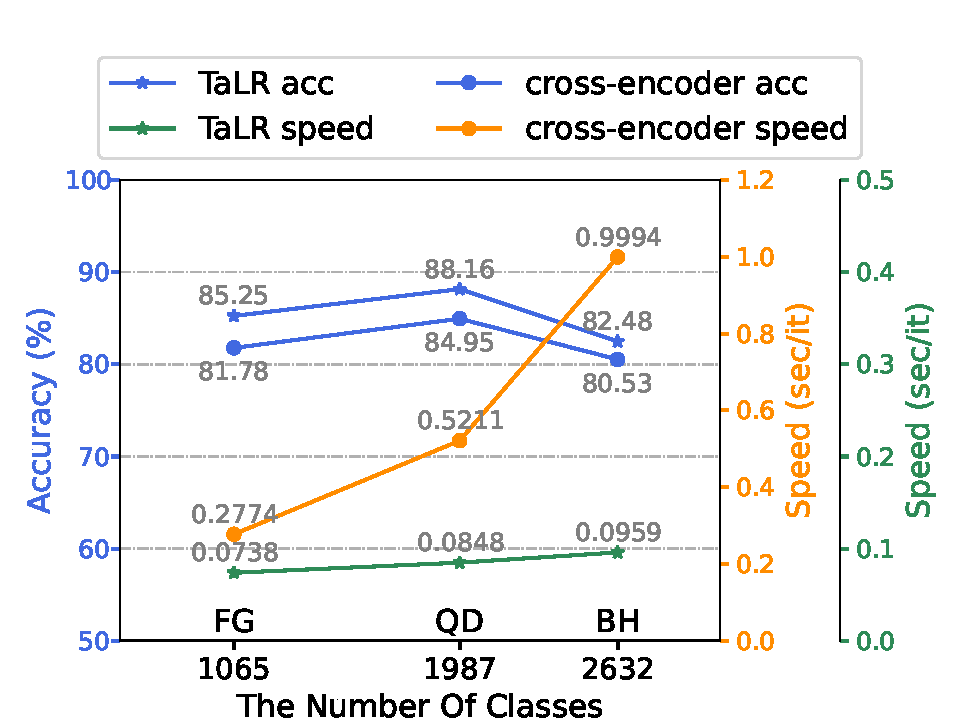
\includegraphics[width=0.4\textwidth]{time.pdf}
    \caption{Accuracy results and inference time consumption when the number of classes grows.} 
    \label{fig:time}
\end{figure}

\subsection{Dynamic Test Set Experiment}
\label{sec:evolve res}
In order to evaluate the ability of our framework on \textbf{taxonomy evolving} challenge, 
we use $\mathsf{TaLR}$ trained on the original multi-domain datasets to directly infer on two dynamic test sets. The vanilla BERT without any finetuning is a naive baseline \textbf{BERT-matching}. The BERT fine-tuned with few-shot new data (1\%) is a strong baseline \textbf{BERT-few-shot}.
% we directly infer product titles with $\mathsf{TaLR}$ trained on multi-domain datasets on the evolved taxonomies.
% we conduct experiments to directly infer evolved new category of the product with $\mathsf{TaLR}$. 
Here ``before'' denotes the subset from the original test set and ``after'' denotes the subset with the same product titles but evolved categories.
From the listed accuracy ``before'' and ``after'' taxonomy evolving in \tabref{tb:evolve}, we can conclude that $\mathsf{TaLR}$ sustains satisfactory accuracy compared with its strong counterpart trained with 1\% extra data.
% the encoded [$\mathtt{CLS}$] token similarity from %%% explained before
% BERT-matching is the vanilla similarity matching baseline and BERT-few-shot is the separate few-shot classifiers we mentioned in \secref{sec: baseline}. Note that BERT-few-shot is trained on full data before evolving.

\begin{table}[th]
\small
\setlength{\tabcolsep}{1.8pt}
  \begin{threeparttable}[b]
  \caption{The accuracy on two dynamic test sets. $\Delta$ is the change
  of accuracy after evolving. The best ``after'' scores and least drop $\Delta$ are bolded.}
  \label{tb:evolve}
  \centering
  \begin{tabular}{l|ccc|ccc}
    \toprule
    \multirow{2}{*}{Methods} & \multicolumn{3}{c|}{QD$-divide$} & \multicolumn{3}{c}{QD$-integrate$}\\
    \cline{2-7}
    & Before & After & $\Delta$ & Before & After & $\Delta$ \\
    \midrule
    BERT-matching & 6.66 & 11.95 & \textbf{+5.29} & 13.39 & 2.23 & -11.16\\
    BERT-few-shot & 90.51 & 43.54 & -46.96 & 86.79 & 50.16 & -36.53\\
    \midrule
    $\mathsf{TaLR}$ & 90.11 & \textbf{69.71} & -20.40 & 85.20 & \textbf{81.48} & \textbf{-3.72}\\
    % (-) contrastive  & 89.10 & \textbf{79.21} & -9.89 & 84.11 & 80.02 & -4.09\\
    % (-) rerank stage & 89.70 & 73.94 & -15.76 & 86.36 & 81.47 & -4.89\\
    % (-) rule-based unit & 89.51 & 64.25 & -25.26 & 84.61 & 81.19 & \textbf{-3.42}\\
    \bottomrule
  \end{tabular}
%   \begin{tablenotes}
%     \item[1] 
%   \end{tablenotes}
  \end{threeparttable}
\end{table}
% {too long, rewrite}
% On the one hand, our $\mathsf{TaLR}$ even outperforms BERT-few-shot without additional training on evolved taxonomies, which indicates its robustness in handling dynamic issues.
% On the other hand, we can observe an opposite trend of BERT-matching and $\mathsf{TaLR}$ through $\Delta$ when two different evolving challenges are encountered. In the node $integrate$ scenarios, $\mathsf{TaLR}$ exhibits robustness with a slight drop of accuracy. 
% When progressively ablating contrastive learning and the whole \textit{Reranking} stage, the accuracy of $\mathsf{TaLR}$ consistently decreases, which indicates their contributions to the node \textit{integrate} variants in evolving taxonomy.
% % \textbf{Taxonomy integration}.
% % On the other hand, BERT-matching suffers from a drastic drop in accuracy, which may attribute to 
% However in the node $divide$ scenario, wherever contrastive learning is incorporated, there is a substantial drop in $\Delta$. Completely excluding the contrastive learning while keeping all other components gives the best accuracy. 
% The reason behind it is that contrastive learning tends to make the representations of products from the same category tied closer, while the division of nodes breaks this relation. 


\subsection{Extrapolating Results on New Taxonomy}
\label{sec:new tax}

% For multi-domain business lines, 
Consider an extreme \textbf{taxonomy evolving} condition when a new business line emerges, a robust model is supposed to categorize incoming products based on the brand-new taxonomy. 
% Hence it poses challenge for $\mathsf{TaLR}$ to zero-shot transfer to new domains so as to improve user experience in this cold-start scenario.

\begin{table}[th]
%   \begin{threeparttable}[b]
  \small
  \caption{The accuracy of $\mathsf{TaLR}$ on the new taxonomy. }
  \label{tb:zeroshot}
  \centering
  \begin{tabular}{l|ccc}
    \toprule
    Methods & QD & BH & FG \\
    \midrule
    BERT-matching & 9.00 & 11.23 & 4.03 \\
    BERT-few-shot & 43.29 & 35.19 & 29.80 \\
    % BERT-product & 52.00 & 48.81 & 51.32 \\
    \midrule
    $\mathsf{TaLR}$ & \textbf{60.57} & \textbf{65.45} & \textbf{62.69}\\
    % $\mathsf{TaLR}$-few(?) &  &  & \\
    % $\mathsf{TaLR}$-finetune(?) & 84.32 & 76.40 & 83.59\\
    % \midrule
    (-) contrastive & 56.71 & 64.99 & 60.79\\
    % (-) Rerank stage & 53.79 & 59.56 & 57.68 \\
    (-) mapping scorer & 56.25 & 64.65 & 59.29\\
    \bottomrule
  \end{tabular}
%   \begin{tablenotes}
%     \item[1] 
%   \end{tablenotes}
%   \end{threeparttable}
\end{table}

We deploy our experiments in a zero-shot manner, where we take turns to train $\mathsf{TaLR}$ on either two business data and test its performance on the remaining business. $\mathsf{TaLR}$ still outperforms BERT-few-shot. 
% We compare $TaLR$ with BERT-matching model and bi-encoder BERT in zero-shot, and $TaLR$-zero sustains better accuracy, 
% This indicates that $\mathsf{TaLR}$'s ability capturing semantic relatedness between product titles and category names on original domains could be seamlessly transferred to new domains with new taxonomies.
This shows $\mathsf{TaLR}$'s preeminent transferability with the reformulation of textual semantic matching, which helps improving user experience in this cold-start scenario.
% It mainly contributes to the learning in the other two domains, 
% which enhances the semantic relatedness understanding in the third dataset with brand new taxonomy.
Each component in the ablation test verifies its effectiveness as well. 

% More details about ablation setting is in \secref{sec:exp detail}.



% \subsection{Different Retrieval Strategies}
% \label{sec:retri stra}
% In \textit{Retrieval} stage, it is encouraged to exploit the potential candidates as accurately as possible, otherwise the latter \textit{Reranking} stage would never make right predictions if the true label is not covered by the retrieved candidates. Hence we use HR@$k$ to measure the retrieval performance.

% Firstly, we compare several alternatives of the loss function in vector-based retrieval model. In \figref{fig:vector-retri}, as $k$ goes on, the HR score increases, and the model trained with Cosent loss is consistently better than others, while the model trained with SBERT loss performs unstably, sometimes worse than Cosine loss. 
% One explanation is that comparing with Cosine loss and SBERT loss, the Cosent loss focuses on the positive-versus-negative pairwise optimization, which means the model only cares for the relative order of the prediction results instead of the specific value. And this setting brings consistent recall of candidates.
% \begin{table}[th]
%   \caption{The retrieval results of the vector-based unit over different loss function. The best results are bolded.}
%   \label{tb:vector-retrieval}
%   \centering
%   \begin{tabular}{c|c|ccc}
%     \toprule
%     Loss & Dataset & HR@1 & HR@5 & HR@10 \\
%     \midrule
%     \multirow{3}{*}{Cosine} & QD & 74.80 & 82.28 & 84.46\\
%     & BH & 72.75 & 81.77& 84.04\\
%     & FG & 65.59 & 80.40 & 83.23\\
%     \midrule
%     \multirow{3}{*}{SBERT} & QD & 82.25 & 88.96 & 90.92\\
%     & BH & 76.95 & 86.76 & 89.41\\
%     & FG & 80.67 & 87.27 & 88.86\\
%     \midrule
%     \multirow{3}{*}{Cosent} & QD & 84.19 & 88.97 & 90.30\\
%     & BH & 77.64 & 85.27 & 87.18\\
%     & FG & 82.72 & 86.66 & 87.48\\
%     \bottomrule
%   \end{tabular}
% \end{table}

% \begin{figure}
%   \begin{subfigure}[b]{0.49\columnwidth}
%   \centering
%   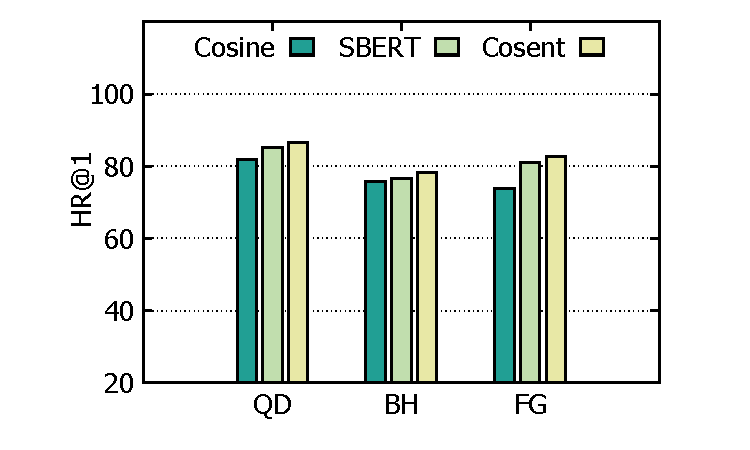
\includegraphics[width=\columnwidth]{hr_1.pdf}
%   \caption{HR@1}
%   \end{subfigure}
% %   \hfill
% %   \begin{subfigure}[b]{0.49\columnwidth}
% %   \centering
% %   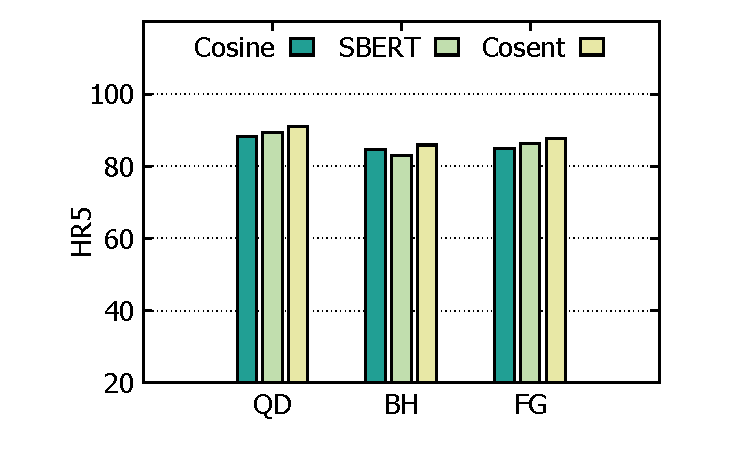
\includegraphics[width=\columnwidth]{hr_5.pdf}
% %   \caption{HR@5}
% %   \end{subfigure}
%   \hfill
%   \begin{subfigure}[b]{0.49\columnwidth}
%   \centering
%   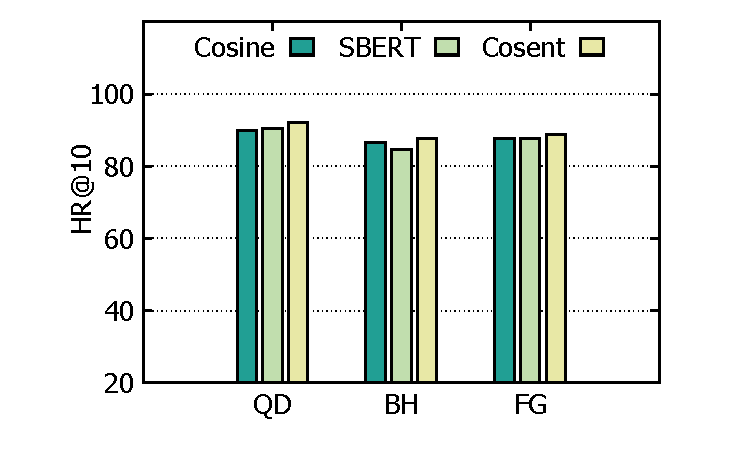
\includegraphics[width=\columnwidth]{hr_10.pdf}
%   \caption{HR@10}
%   \end{subfigure}
%   \caption{The retrieval results of the vector-based unit over different loss functions.}
%   \label{fig:vector-retri}
% \end{figure}

\cut{
To generate better candidates, we adopt several heuristic algorithms for two-way candidates fusion.
% the vector-based unit and rule-based unit. 
\tabref{tb:fusion} depicts the retrieval results over different fusion strategies. The size of merged candidate sets is not stuck to $10$ for some of the strategies, so we list the average number.
Generally, the \textbf{Rule-First} algorithm achieves better scores, and \textbf{De-Dupli} algorithm is competitive with it. We use \textbf{Rule-First} in our framework due to its fixed candidate size which is more convenient to process.
Although the pure vector-based unit performs less effectively than the rule-based counterpart, they could complement each other after fusing together with the help of an ensembled understanding of textual semantics and training set distribution.
% the ensemble of vector-based unit and rule-based unit strengthens the performance of rule-based unit, revealing that vector-based unit can better understand the instance semantically that rule-base unit can not. 
More discussions are in Case Study.

\begin{table}[th]
\setlength{\tabcolsep}{2pt}
  \caption{The retrieval results of candidates for different fusion strategies. The best results are bolded.}
  \label{tb:fusion}
  \centering
  \begin{tabular}{c|cc|cc|cc}
    \toprule
    \multirow{2}{*}{Strategy}  & \multicolumn{2}{c|}{QD} & \multicolumn{2}{c|}{BH} & \multicolumn{2}{c}{FG} \\
    \cline{2-7} 
      & Recall & Size & Recall & Size & Recall & Size \\
    \midrule
    Rule-based & 95.33 & 8.6 & 96.77 & 8.8 & 97.32 & 9.0 \\
    Vec-based & 90.30 & 10 & 87.18 & 10 & 87.48 & 10 \\
    \midrule
    De-Dupli & 96.08 & 10.5 & \textbf{97.54} & 10.4 & 97.77 & 10.7 \\
    Norm\&Rank & 93.74 & 10 & 92.42 & 10 & 92.77 & 10 \\
    Rule-First & \textbf{96.12} & 10 & 97.48 & 10 & \textbf{98.01} & 10 \\
    \bottomrule
  \end{tabular}
\end{table}
}
% \section{Case Study}
% For product ``\textit{red dancing shoes (size 35)}'', which should be categorized to \verb|Sports/Outdoors| $\rightarrow$ \verb|Yoga/Dancing| $\rightarrow$ \verb|Dancing Shoes|, the vector-based unit retrieves the correct class as top-$1$ answer, but the rule-base unit retrieves \verb|Clothes/Shoes| $\rightarrow$ \verb|Woman Shoes| $\rightarrow$ \verb|Woman Slippers| as top-$1$. This time the distribution knowledge guides the rule-based model towards a wrong direction, while the vector-based model succeeds relying on the semantic similarity.

% For product ``\textit{CHEERS$^\circledR$ 12 years}'', the vector-based model categorizes it to \verb|Books| $\rightarrow$ \verb|Economics/Management| $\rightarrow$ \verb|Marketing|, whereas the rule-based unit correctly retrieves \verb|Alcoholic Drinks| $\rightarrow$ \verb|Imported Liquors| $\rightarrow$ \verb|Whisky|. This shows that ``12 years'' misleads the vector-based model to the semantic meaning of economics, and rule-based unit successfully leverages its distribution knowledge in training set.

% For product ``\textit{towel gourd\&soy bean (towel gourd 1 pcs, soy bean 150g)}'', both rule-based unit and vector-based unit predict
% \verb|Vegetable| $\rightarrow$ \verb|Soy Product| $\rightarrow$ \verb|Soy Bean| wrongly as top-$1$, whereas $\mathsf{TaLR}$ classifies it to correct \verb|Vegetable| $\rightarrow$ \verb|Mixed Product| $\rightarrow$ \texttt{Vegetables mixture}, and clearly, the contribution is from the following \textit{Reranking} stage.
% \begin{table*}[t]
%   \caption{The retrieval results of candidates for different fusion strategies. The best results are bolded.}
%   \label{tb:fusion}
%   \centering
%   \begin{tabular}{c|c}
%     \toprule
%     Product title & \textit{red dancing shoes (size 35)} \\
%     \midrule
%     Ground truth & \verb|Sports/Outdoors| $\rightarrow$ \verb|Yoga/Dancing| $\rightarrow$ \verb|Dancing Shoes| \\
%     Vector-based top-$1$ & \verb|Sports/Outdoors| $\rightarrow$ \verb|Yoga/Dancing| $\rightarrow$ \verb|Dancing Shoes| \\
%     Rule-based top-$1$ & \verb|Clothes/Shoes| $\rightarrow$ \verb|Woman Shoes| $\rightarrow$ \verb|Woman Slippers| \\
%     \midrule
%     Product title & \textit{CHEERS$^\circledR$ 12 years} \\
%     \midrule
%     Ground truth & \verb|Alcoholic Drinks| $\rightarrow$ \verb|Imported Liquors| $\rightarrow$ \verb|Whisky| \\
%     Vector-based top-$1$ & \verb|Books| $\rightarrow$ \verb|Economics/Management| $\rightarrow$ \verb|Marketing| \\
%     Rule-based top-$1$ & \verb|Alcoholic Drinks| $\rightarrow$ \verb|Imported Liquors| $\rightarrow$ \verb|Whisky| \\
%     \midrule
%     Product title & \textit{towel gourd \& soy bean (towel gourd 1 pcs, soy bean ~150g)} \\
%     \midrule
%     Ground truth & \verb|Vegetable&/ Product| $\rightarrow$ \verb|Mixed Product| $\rightarrow$ \verb|Vegetables mixture| \\
%     Vector-based top-$1$ & \verb|Vegetable/&Soy Product| $\rightarrow$ \verb|Soy Product| $\rightarrow$ \verb|Soy Bean| \\
%     Rule-based top-$1$ & \verb|Vegetable/Soy Product| $\rightarrow$ \verb|Soy Product| $\rightarrow$ \verb|Soy Bean| \\
%     \bottomrule
%   \end{tabular}
% \end{table*}



\subsection{Online Experiment}
% We conduct online experiments on one downstream task where the category of a product is needed, 
% % of semantic vector space, 
% that is the main page recommendation (multi-domain). 
% % After deploying our contrastive pretrained model to compute the hidden vector representations of related products and utilizing this in sophisticated 
% When $\mathsf{TaLR}$ is incorporated in the
% recommendation system, customer purchase click rate increases significantly over 5\%.
We conduct online experiments on one downstream task where $\mathsf{TaLR}$'s domain-independent category recognition ability helps transfer user preferences from other domains and contributes to a more accurate recommendation. When $\mathsf{TaLR}$ is incorporated in the recommendation system, customer seasonal purchase revenue increases significantly over 5\%.
\section{Related Work}
\paragraph{Clarification Question Generation} The concept of CQ can be naturally raised in a dialogue system where the speech recognition results tend to be erroneous so that we raise CQs for sanity check \citep{stoyanchev2014towards}, or the intents for a task is incomplete or ambiguous in a first short utterance and further CQs are needed to fill in the slots \citep{dhole2020resolving}. The concept is then extended to IR to clarify ambiguous queries \citep{aliannejadi2019asking}, and has been successfully put into practice \citep{zamani2020generating}. Other application areas including KBQA \citep{xu2019asking} and open-domain dialogue systems \citep{aliannejadi2020convai3}. CQGen can also be applied to help refine posts on websites like StackExchange \citep{Kumar_2020} and Amazon \citep{rao2019answer}. In this context, our work closely follows the research line of \citep{rao2018learning, rao2019answer, cao2019controlling}. \citet{rao2018learning} first adopted a retrieval-then-rank approach. They \citep{rao2019answer} then proposed a generation approach to train the model to maximize the utility of the hypothetical answer for the questions with GAN, to better promote specificity. \citet{cao2019controlling} propose to control the specificity by training on data with explicit indicator of specificity, but it requires additional specificity annotation. Towards the similar specificity goal, we adopted a different keyword-based approach. They also assume generating one question per context, which we claim is not sufficient to cover various possible information needs, and thus propose the task of the diverse CQGen.

\paragraph{Diverse Generation} The demand for diverse generation exists in many other fields~\cite{vijayakumar2018diverse, LiangZ18code, shen2019mixture}, and we've drawn inspirations from these literatures. For image captioning, we may use multiple descriptions for different focusing points of a scene. \textit{Diverse Beam Search} \citep{vijayakumar2018diverse} was proposed to broaden the searching space to catch such diversity by dividing groups in decoding and imposing repetition penalty between them. For machine translation, a context can be translated with different styles. \citet{shen2019mixture} thus proposed \textit{Mixture of Expert} models including hMup to reflect various styles with a discrete latent variable (\textit{expert}). And here for CQGen, diversity is required to cover various potentially missing aspects, so we come up with the idea to use keywords as a controlling variable like \textit{expert} to promote diversity.


\section{Conclusion}

In this paper, we incorporated the idea of Cookie Theft picture description task into the evaluation of the high-level cognitive abilities of LVLMs and designed a novel evaluation benchmark called CogBench.
% Images in CogBench are of high quality and require more cognitive reasonings to understand, which makes it different from existing image datasets.
The images in CogBench are of high quality and demand more complex cognitive reasoning for interpretation, setting it apart from existing image datasets.
% It consists of a image description task and a VQA task.
Experiments show that there is still a large gap between the cognitive abilities of LVLMs and human beings, indicating CogBench is a challenging benchmark.

% In the future


% Use \bibliography{yourbibfile} instead or the References section will not appear in your paper
% \nobibliography{aaai22}
\bibliography{sample-base}

% \section{Acknowledgments}

\end{document}
